\documentclass[10pt]{aastex62}
\usepackage{amsmath,amssymb,lmodern,mathrsfs,ulem,mathtools, bm}
\usepackage{graphicx}
\usepackage{enumitem}
\usepackage{natbib}
\usepackage{xcolor}

%%%%%%%%%%%%%%%%%%%%%%%%%%
%%%%
%%%%   Custom commands for special characters.
%%%%
%%%%%%%%%%%%%%%%%%%%%%%%%%

%bold-face nabla symbol for gradients
\newcommand{\grad}{\mbox{\boldmath$\nabla$}}
%upright derivative symbol
\newcommand{\dd}{\mathrm{d}}
%raised phi to compliment raised chi
\newcommand{\rphi}{\mathpalette\raisephi\relax}
\newcommand{\raisephi}[2]{\raisebox{\depth}{$#1\varphi$}}
%raised chi looks better in fractions
\newcommand{\rchi}{\mathpalette\raisechi\relax}
\newcommand{\raisechi}[2]{\raisebox{\depth}{$#1\chi$}}

%%%%%%%%%%%%%%%%%%%%%%%%%%
%%%%%
%%%%%     Custom colors for editorial comments
%%%%%
%%%%%%%%%%%%%%%%%%%%%%%%%%

\definecolor{forest}{RGB}{34,139,34}
\definecolor{lime}{RGB}{50,205,50}
\newcommand{\tr}[1]{{\color{red} #1}}
\newcommand{\tb}[1]{{\color{blue} #1}}
\newcommand{\tg}[1]{{\color{lime} #1}}



\watermark{DRAFT}
\setwatermarkfontsize{2cm} 

\begin{document}

\received{May, 2018}
\revised{\today}
%\accepted{-- ~}
%\published{--}
%\submitjournal{}

\title{\path{HQVseg}: A python module for discretizing coronal magnetic domains.}
\author[0000-0001-8517-4920]{Roger B. Scott} % https://orcid.org/0000-0001-8517-4920
\affiliation{School of Science and Engineering, University of Dundee, Dundee DD1 4HN, UK}

\correspondingauthor{Roger B. Scott}
\email{roger.b.scott@gmail.com}

\begin{abstract}
In order to understand the topology of coronal magnetic field models it is useful to have a method for partitioning the coronal volume into discrete magnetic flux domains.
This can be accomplished by finding all of the magnetic nulls in the volume and then tracing their fan and spine field lines; however, this process is quite laborious and computationally intensive.
Additionally, while the magnetic skeleton is, in principle, a complete representation of all topological features, there are morphological features such as hyperbolic flux-tubes, which can be important for magnetic reconnection, that are not captured by this method.
An alternative approach is to calculate the magnetic squashing factor and use this to identify so-called quasi-separatrix layers, which can be sites of 3D magnetic reconnection without the presence of magnetic nulls.
Because the magnetic squashing factor is scalar quantity that is conserved along a given field line, its isosurfaces are equivalent to magnetic flux tubes, and can therefore be used is indicators of magnetic flux domains.
Here we describe a domain segmentation routine that discretises the coronal volume using the magnetic squashing factor as a proxy for topological boundaries.
This method draws heavily on methodology developed for image processing and 3D medical imaging, but is entirely open source and depends only on publicly available image analysis libraries.
\\
\end{abstract}

\section{Code Summary}\label{summary.sec}

The strategy of this routine is as follows:
\begin{itemize}
\item[1]{The magnetic field model and calculated values for the magnetic squashing factor are read in from disc, and their numerical representations are reconciled to a single grid.}
\item[2]{A mask is created based on thresholding of the magnetic squashing factor and its gradient. The mask is then padded and holes are removed to ensure that it is `water tight'.}
\item[3]{The unmasked volume is partitioned into discrete domains, each with a unique label -- the discretisation is performed separately for open and closed field regions to ensure that the open and closed boundary is not spanned by any single domain.}
\item[4]{The masked region is then labeled using a watershed segmentation, which allows each region to compete for the volume previously occupied by the mask, so that the various regions collectively span the entire coronal volume.}
\item[5]{The masked volume is then sorted based on proximity to the various discrete domains, with the interfaces between these domains indicating the location of topological and morphological features.}
\item[6]{Finally, the various subsets of the masked volume are tagged and sorted based on their proximity to each other and to nulls in the magnetic field, so that the inferences can be made regarding the typical rates of occurrence of the various types.}
\end{itemize}

In order to execute this strategy we have created a self-contained \path{Python} module \path{HQVseg}, whose methods and classes are described in detail below.
This module depends on a number of other publicly available \path{Python} modules, such as \path{NumPy}, \path{SciPy} \citep{SciPy}, \path{Scikit-Image} \citep{scikit-image}, \path{ndimage}, to name a few.
The hierarchy of classes and their methods is given below, with more detailed descriptions in subsequent sections.

\begin{itemize}
	\item{module: \path{HQVseg}
		\begin{itemize}
			\item{class: \path{Inputs()}}
			\item{class: \path{Source()}}
			\item{class: \path{Result()}}
			\item{class: \path{Model()} 
					\begin{itemize}
						\item{subclasses: \path{Inputs(), Source(), Result()}}
						\item{setup methods: \path{build_grid(), import_squash_data(), import_bfield_data()}}
						\item{segmentation methods: \path{build_masks(), segment_volume()}}
						\item{metadata methods: \path{determine_adjacency(), find_interior_HQVs(), find_exterior_HQVs(), get_null_region_dist(), get_null_intHQV_dist(), associate_structures(), categorize_structures()}}
						\item{support methods: \path{global_reduce(), global_expand(), associate_labels(), get_reg_hqv(), get_reg_bnd(), make_null_box(), get_null_regs()}}
						\item{data i/o methods: \path{cloan(), save_data(), load_data(), export_vtk()}}
						\item{visualization methods: \path{gauss_slice(), segcmap(), mskcmap(), visualize()}}
					\end{itemize}}
			\item{class: \path{Foo()}}
			\item{class: \path{Bytefile()}}
			\item{method: \path{portattr()}}
			\item{method: \path{get_mask_boundary()}}
		\end{itemize}}
\end{itemize}

The primary wrapper for handling data and related calculations is the \path{Model()} object class, whose methods and attributes define the main scope of the module.
Within this main class there are three additional object classes that contain the data, metadata, and results from the segmentation calculation.
These are classes of the module at large but their primary functionality is as attributes of the larger model class.
The contents of these data objects is as follows:

\begin{itemize}

\item{\path{Model().Inputs():} \begin{itemize}
\item{Object class containing default values, filenames, and other initialization data.}
\item{Updated dynamically as various routines check for and subsequently set default values.}
\item{Attributes: \path{nrr, nth, nph, phmin, phmax, thmin, thmax, rrmin, rrmax, r_samp, solrad, q_dir, b_dir, glbl_mdl, ss_eof, sbn_thrsh, ltq_thrsh, adj_thrsh, pad_ratio, bot_rad, auto_imp, auto_seg, protocol, vis_title, initialization}}
\end{itemize}
}

\item{\path{Model().Source():}\begin{itemize}
\item{Object class containing source magnetic field data and numerical grid.}
\item{Populated by execution of setup methods.}
\item{Attributes: \path{crr, cth, cph, brr, bth, bph, slog10q, metrr, metth, metph, null_locs}.}
\end{itemize}
}

\item{\path{Model().Result():}\begin{itemize}
\item{Object class containing data generated by segmentation routines and subsequent post-processing.}
\item{Populated by execution of segmentation methods and metadata methods.}
\item{Attributes: \path{hqv_msk, PIL_msk, GlnQp, reg_width, hqv_width, pad_msk, vol_seg, seg_msk, labels, open_labels, clsd_labels, opos_labels, oneg_labels, adj_msk, adj_msk_shape, adj_msk_boolsize, exterior_HQVs, interior_HQVs, null_info, null_to_region_dist, null_to_intHQV_dist}.}
\end{itemize}
}

\section{Setup}

Setting up the model consists of reading in data from disc, constructing the numerical grid, and reconciling the magnetic field data to the finer resolution grid of the squashing factor data.
Squashing factor data is output from the post-processed \path{qslSquasher} code, for which the data is stored in a flattened datafile with no coordinate information.
As such, the grid is first built (\path{Model().build_grid()}) by assuming typical limits and resolution to the coordinate domain, consistent with the definition used in the \path{qslSquasher} routines.
The squashing factor ($Q$) data is then read in (\path{Model().import_squash_data()}) and reshaped to match the grid dimensions.
The source magnetic field ($\bm{B}$) data is then read in (\path{Model().import_bfield_data()}) along with the associated coordinate axes, and then interpolated onto the appropriate grid.

The routines used assume by default that the data is in a particular format; however, these should be readily extensible to variations in formatting, either through changes to keywords or restructuring of the code.
The default functionality of these routines is given below.

\begin{figure}
\center
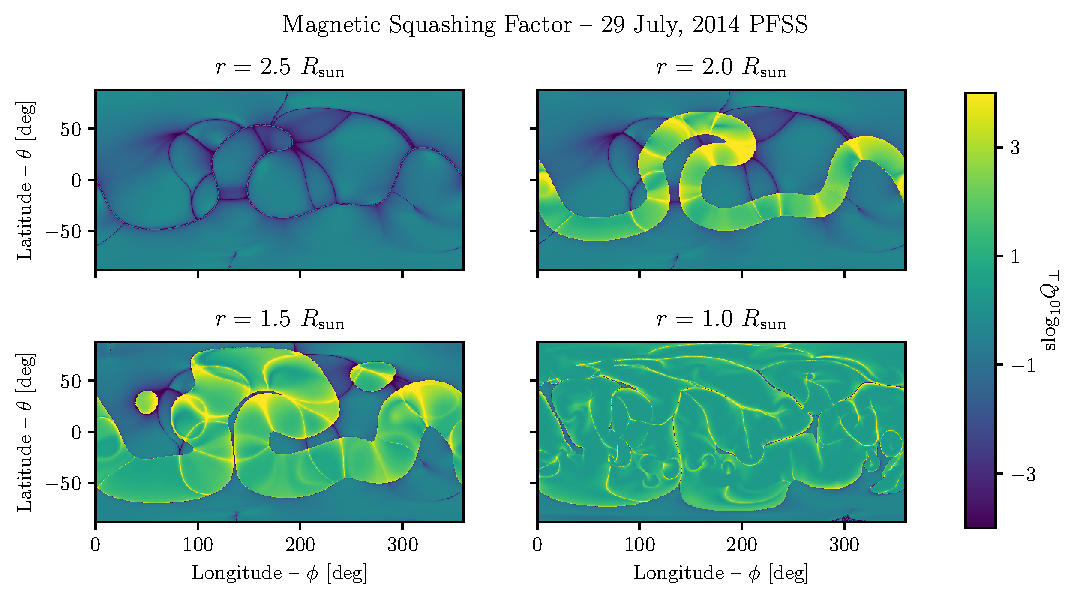
\includegraphics[width=\linewidth]{./fig_src_fls/140729_slog10q_multi.pdf}
\caption{Sign $\log_{10} Q$ at radial heights of $r = \{1.0, 1.5, 2.0, 2.5\} R_{\rm sun}$ for 29 July, 2014 PFSS. Dark colors indicate open flux, corresponding to coronal holes at the lower boundary. Dark bands at the upper boundary indicate the intersections of QSLs with the source surface. The yellow curve in the top panel shows the apex of the helmet streamer, just below the heliospheric current sheet.}
\label{slog10q_multi.fig}
\end{figure}

The \path{Model().build_grid()} method assumes a default configuration of $\text{\path{nrr}}=120$, $\text{\path{nth}}=4~\text{\path{nrr}}$, $\text{\path{nph}}=8~\text{\path{nrr}}$, with coordinates spaced evenly in $0 \le \ln(r / R_\odot) \le \ln(2.5)$, $-88^\circ \le \theta \le 88^\circ$, $0 \le \phi \le 360^\circ$.  
The value of $R_\odot$ is set explicitly to \path{inputs.solrad}=$696$ and the resulting coordinate grid is a finite difference mesh with coordinates written to the variables \path{source.crr}, \path{source.cth}, \path{source.cph}. 
Coordinate gradients (diagonal metric entries) are also calculated and written to \path{source.metrr}, \path{source.metth}, \path{source.metph}. 

With the grid in place, the \path{Model().import_squash_data()} method assumes that the squashing factor data are stored in a file called \path{q_dir/grid3d.dat}, where \path{q_dir} is an attribute of \path{Model().inputs} and is set during instantiation.
The data is assumed to have the dimensions defined in \path{Model().build_grid()}, and is written as a nested loop of the form given in \cite{Tassev:2016}. 
If \path{inputs.q_dir} is not set explicitly, the current working directory is inspected for the appropriate file. 
Once the data are read in to memory they are stored in the variable \path{source.slog10q}, which is assumed to correspond to the ${\rm slog}_{10} Q_\perp$ representation from \cite{Scott:2018a}

\begin{figure}[h]
\center
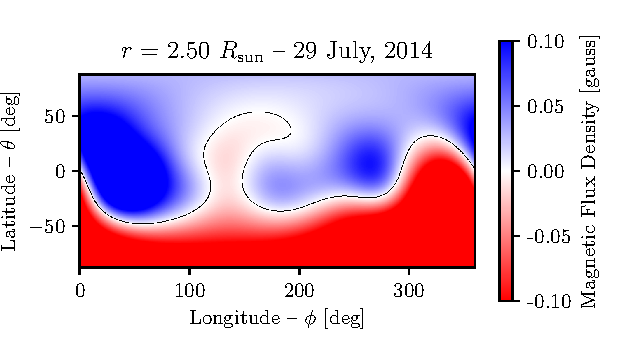
\includegraphics[width=0.45\linewidth]{./fig_src_fls/140729_br_top.pdf}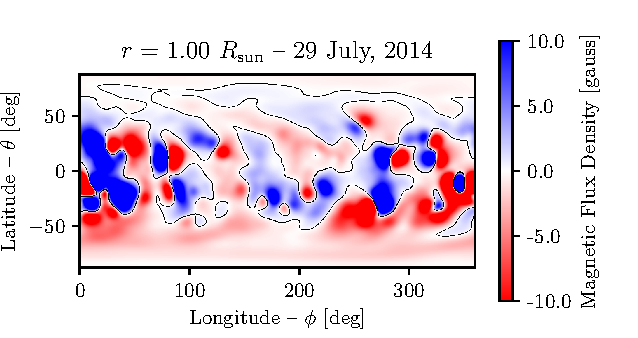
\includegraphics[width=0.45\linewidth]{./fig_src_fls/140729_br_bot.pdf}
\caption{Radial magnetic field ${\bf B}^{(8)}$ from 29 July 2014. The top and bottom panels represent the source surface ($r=2.5 R_{\rm sun}$) and photospheric ($r=1.0 R_{\rm sun}$) boundaries. Data is smoothed with a  pseudo-gaussian filter of the form $f = exp(-l(l+1) k)$, with $k=0.002$. The field is then interpolated onto a grid with the same dimensions as $Q$ (see section \ref{squash.sub}) for consistency. }
\label{source_field.fig}
\end{figure}

The \path{Model().import_bfield_data()} method assumes that the magnetic field data are stored in a collection of files \path{b_dir/bx0.dat}, \path{b_dir/by0.dat}, \path{b_dir/bz0.dat}, with corresponding coordinate axes in \path{b_dir/xs0.dat}, \path{b_dir/ys0.dat}, \path{b_dir/zs0.dat}.
As above, \path{b_dir} is an option stored in \path{inputs.b_dir} and is set, by default, to be \path{b_dir}=\path{q_dir+bfield_data/}.
Consistent with the convention used in \path{qslSquasher}, the $x, y, z$ variable are taken as proxies for $\phi, \theta, r$ in spherical coordinates. 
The data are assumed to be unrolled in the same fashion as \path{slog10q}. 
Interpolating functions are then generated assuming a regular grid and the data are then interpolated onto the same grid as \path{slog10q}, and the original data are discarded.
The interpolated values of the magnetic field are stored at \path{source.brr}, \path{source.bth}, \path{source.bph}. 
Additionally, data indicating the number and location of magnetic nulls, which are calculated separately and stored in \path{b_dir/nullpositions.dat}, are imported at this step if available.


\section{Segmetation}

The actual volume segmentation is performed in combination between two methods of the \path{Model()} class, \path{Model().build_hqv_msk()} and \path{Model().segment_volume()}. 
The first method is a standalone routine that constructs a mask for identifying so-called High Q Volumes (HQVs). 
The routine first recovers the perpendicular squashing factor from the array of stored values as $Q_\perp = 10^\wedge |{\rm slog10q}|$.
The (radius-normalized) squared Sobolev norm is then constructed as
\begin{equation}
N_{S}^2 = Q_\perp + \frac{r}{R_\odot}{\grad_r}\ln(Q_\perp),
\end{equation}
where $r$ and $R_\odot$ are the local radius and solar radii, respectively, and ${\grad_r}$ is the numerical gradient vector, normalized to the local value of $r$. 

Since $Q_\perp$ is formally infinite at various places in the domain, $N_S^2$ has no well defined mean; however, we can compute a proxy for the typical value of $N_S^2$ as 
\begin{equation}
\tilde{N}_S^2 = \sqrt{\left < \left (2 + \frac{r}{R_\odot}{\grad_r}\ln Q_\perp \right )^2 \right >},
\end{equation}
where $Q_\perp$ has been replaced by its theoretical minimum value of 2. 
With this characteristic value we can then define the High Q Volume as a subset of the larger domain given by 
\begin{equation}
\Omega_{\rm HQV} = \left \{{\bf x} \in \Omega \quad | \quad \left ( N_S^2({\bf x}) > 1.5\, \tilde{N}_S^2 \quad \text{or} \quad \log_{10}Q_\perp > 3.7 \right ) \right \},
\end{equation}
which is stored as a mask according to the boolean
\begin{equation}
\text{\path{hqv_msk}}_{ij} = \left ( 1 \quad \text{if} \quad {\bf x}_{ij} \in \Omega_{\rm HQV}\quad , \qquad 0 \quad \text{else} \right ).
\end{equation}

The \path{Model().build_hqv_msk()} method makes no strict assumptions about the grid but does assume that positive (negative) values of \path{slog10q} correspond to closed (open) magnetic flux domains. 
The gradient thresholding described above is performed using built-in \path{numpy} routines and the mask is smoothed using morphological opening and closing from the \path{scikit-image.morphology} package.
Defaults for the thresholding are stored in \path{inputs.ltq_thrsh} and \path{inputs.sbn_thrsh}, and can be specified separately prior to execution.
The resultant mask is stored in \path{result.hqv_msk} and $\grad_r \ln Q_\perp$ is stored at \path{inputs.GlnQp} for diagnostic purposes.

Following the creation of the \path{hqv_msk}, the volume is then discretized using the \path{Model().segment_volume()} routine, which is built on the operating assumption that domain boundaries should lie within $\Omega_{\rm HQV}$ and be locally perpendicular to $\grad Q_\perp$. 
The segmentation is performed in a number of steps that are designed to minimize the possibility of separate flux domains having a common label, especially across the open-closed boundary. 
Note that while the visuals provided here are indicative of the behavior at the top boundary, the segmentation is fully-3D and includes open and closed flux, throughout the volume.

Prior to segmenting the volume, we first consider whether the azimuthal boundary is meant to be periodic, in the case of a global model (\path{inputs.glb_mdl}). 
If it is, we first expand the \path{hqv_msk} and \path{slog10q} arrays to double their azimuthal extent, by stacking to adjacent versions of these, and then sliding by $180^\circ$ in $\phi$. 
This is done to place the periodic, azimuthal boundary, within the interior of the numerical domain, so that it will be transparent to the subsequent segmentation.
A future improvement to this method would simplify this process by incorporating periodicity directly into the underlying segmentation routines, which do not support periodicity in their standard form.

The first step in the segmentation is to pad the mask to ensure that there are no `leaks' from numerical artefacts.
This is accomplished by calculating the euclidean distance transform (\path{scipy.ndimage.distance_transform_edt}) to determine the distance of all non-HQV points to the nearest element of $\Omega_{\rm HQV}$. 
This value is stored in \path{hqv_dist} and a new mask, \path{pad_msk}, is then constructed to reflect all points with \path{hqv_dist} greater than a threshold value. 
The threshold is set by calculating the distance transform for the compliment of $\Omega_{\rm HQV}$, from which we get the mean linear width of a typical HQV element, which is stored at \path{hqv_width}.
The \path{pad_msk} variable is then used to discretely label all unique, simply connected domains, using the \path{skimage.measure.label} method, which assigns a unique integer label to all pixels within each unique domain.
This labling is performed separately for open and closed domains, which are assigned positive (negative) labels consistent with the convention for \path{slog10q}. 
The combined label array is stored as \path{vol_seg}, which is an integer array of the same size as \path{slog10q}.

Following the initial labeling, we must still assign domain labels to the HQV volume, as we intend for the various domains to completely span the numerical domain eventually.
The intention is that the HQV regions should be assigned labels from adjacent low-Q regions so that eventually each label corresponds to a region with low-Q in its interior and high-Q only and exactly at the interfaces between adjacent regions.
To accomplish this, we use the \path{skimage.morphology.watershed} routine, which takes a collection of seed values, and populates unmasked pixels with seed values consistent with a watershed-basin model. 

If unchecked, the method will populate the entire domain; however, we wish to enforce certain constraints on how the regions are grown, so the watershed is performed in a series of individual steps, with the mask peeled away in stages.
At the outset, we remove any domains with a volume below a threshold value, as these tend to be single-pixel domains and are taken to be artefacts.
We then proceed with the expansion of remaining regions, and in the following, each step is always performed twice, once for open domain, and once for closed domains, so as to ensure that open flux is never assigned to a closed flux domain, and visa-versa. 
First, the padded buffer is backfilled with a watershed growth into the unlabled pixels in \path{pad_msk} but not in \path{hqv_msk} and a same-type-only (e.g., open or closed) mask is used to ensure contiguous growth.
Second, the watershed is performed on unlabled pixels within the \path{hqv_msk}, again with a same-type-only contiguous growth mask, to fill smooth, non-pathological elements of the HQV. 
Third, we repeat the watershed on unlabled pixels in the \path{hqv_msk} but now without contiguous growth, as we recognize that domains can appear to be pinched off when they are in fact connected below the grid resolution.
And finally, we remove all masks and label as-yet unlabled pixels, to allow for population of junk data-values where the flux could not be accurately reported as strictly open or closed.

After segmenting the volume, we must still reconcile the periodicity of the domains in the case of a global model.
As the labeling was performed with an artificially enlarged domain, the azimuthal boundaries are placed within the interior of the numerical domain during segmetnation, so there are no discontinuities at these locations;
however, it remains that the labels on the left side of the domain are different than their counterparts on the right side. 
To rectify this we use another routine, \path{Model().associate_labels()}, which breaks to domain into its two adjacent copies, and then compares their labels pairwise to look for overlaps.
Once the overlaps are identified, the domains are iteratively renamed and the pairwise matches updated, until all overlaps have been reconciled. 
The domain labels are then reduced to a compact, monotonic set, with missing elements removed, and are classed based on whether the flux is open or closed, with open flux further subdivided into two groups based on the sign of the magnetic field at the top boundary.
Once the domains have been relabeled, the domain extent is reduced to the original grid and the label map is written to \path{result.vol_seg} with the various lists of different typed labels recorded as \path{result.labels, result.clsd_labels, result.open_labels, result.opos_labels, result.oneg_labels}. 


\begin{figure}
\center
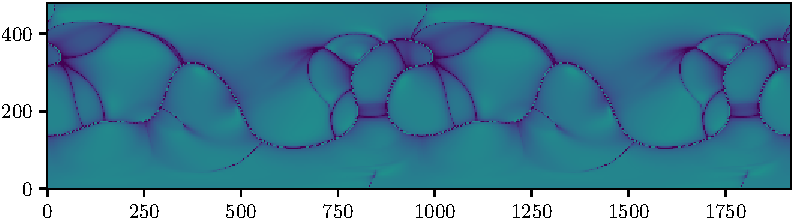
\includegraphics[width=0.45\linewidth]{./fig_src_fls/seg0}\hspace{0.1in}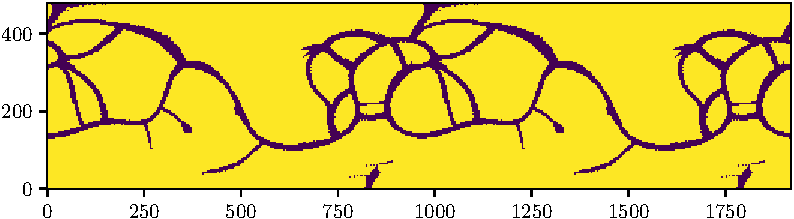
\includegraphics[width=0.45\linewidth]{./fig_src_fls/seg1}\\
\vspace{0.1in}
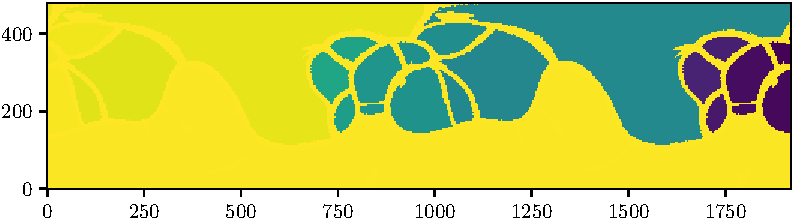
\includegraphics[width=0.45\linewidth]{./fig_src_fls/seg2}\hspace{0.1in}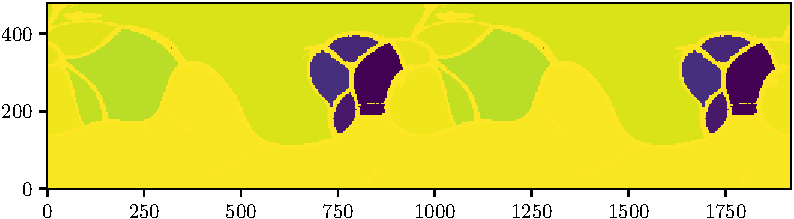
\includegraphics[width=0.45\linewidth]{./fig_src_fls/seg3}\\
\vspace{0.1in}
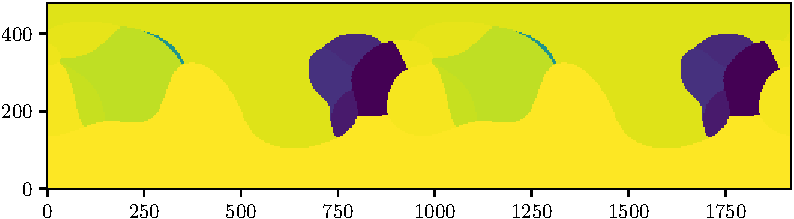
\includegraphics[width=0.45\linewidth]{./fig_src_fls/seg4}\hspace{0.1in}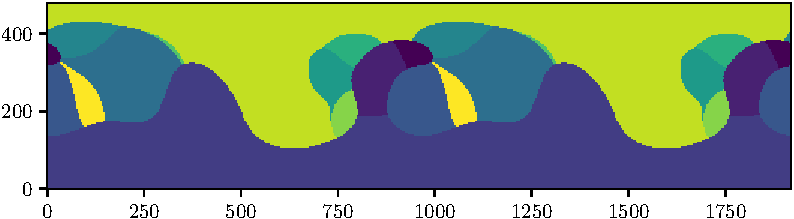
\includegraphics[width=0.45\linewidth]{./fig_src_fls/seg5}
\caption{Stages of volume segmentation: raw $Q_\perp$ map (tl), HQV mask (tr), discrete labeling (cl), periodic relabeling (cr), backfilling (bl), label reduction (br).}
\label{seg_steps.fig}
\end{figure}

\section{HQV Identification}

In order to identify which portions of the high-Q volume lie at the interfaces of specific domains, we must find the distance from each point in the volume to nearest portion of given domain. 
This is accomplished by the routine \path{Model().determine_adjacency()}, which loops over all possible domain labels and calculates the distance from every point in the volume to the nearest point in a given domain according the the \path{scipy.ndimage.distance_transform_edt()} routine. 
The resultant value is compared to a threshold value, which is set by default to be equal to \path{result.hqv_width} in the middle of the domain, and scales with the local radius. 
The collection of all points whose distance to a given domain is less than the threshold value are said to be adjacent to the domain, and this information is stored as a boolean map.
The ensemble information for all domains is boolean array called \path{result.adj_msk}, with dimension $\left ( \text{\path{nrr}} \times \text{\path{nth}} \times \text{\path{nph}} \times \text{\path{n_regs}} \right )$, where \path{n_regs} is the total number of discrete domains, stored at \path{result.n_regs}. 

Because \texttt{Python} stores boolean as an integer type, \path{result.adj_msk} is quite large in practice, so for practical reasons it is compressed to a bitwise array when storing to disc.
The adjacency mask is used directly by the \path{Model().get_reg_hqv()} routine, which returns a mask corresponding to all pixels that lie within the larger \path{hqv_msk} and also identify as adjacent to whichever domain is specified. 
If more than one domain is specified the result is either the intersection (default) or union of the individual entries. 
By testing for the existence of non-empty intersection groups with various domain pairings, a list of all non-trivial interface HQVs is formed using the routine \path{Model().find_exteriorHQVs()}.
The result of this testing is an attribute called \path{result.exterior_HQVs}, which is a list whose entries are objects containing the various metadatum about each pairing.

The collection of \path{exterior_HQVs} necessarily omits any high-Q volume that is contained entirely within a single domain, so an additional routine is required to identify such structures.
This is accomplished by a routine called \path{model.find_interiorHQVs()}, which loops through each domain and identifies portions of the \path{hqv_msk} that associates with that domain and no other.
These sub-volumes are then inspected for contiguous structures, which are labeled and filtered against a size threshold, after which surviving elements are allowed to expand back to the domain boundary using a simplified version of the same watershed technique used for the larger segmentation. 
The result of this search is another attribute called \path{result.interior_HQVs}, which again is a list whose entries are objects with attributes containing metadatum about the various unique, non-interface high-Q volumes. 

The final result of this sorting of high-Q sub-volumes is a pair of lists containing masks (or pointers to masks) and metadata for every non-trivial high-Q structure, catalogued according to the specific flux-domains to which they are adjacent.
In the case of \path{result.exterior_HQVs}, each entry contains a list of labels, and the corresponding high-Q volume is constructed by passing this list as an argument to \path{Model().get_reg_hqv()}.
In the case of \path{result.interior_HQVs}, since a given domain can contain multiple separate high-Q volumes within it's interior, each entry contains a label number and a sub-label number, along with a boolean mask for that specific high-Q structure. 

\section{HQV Inspection}

\begin{figure}
\center
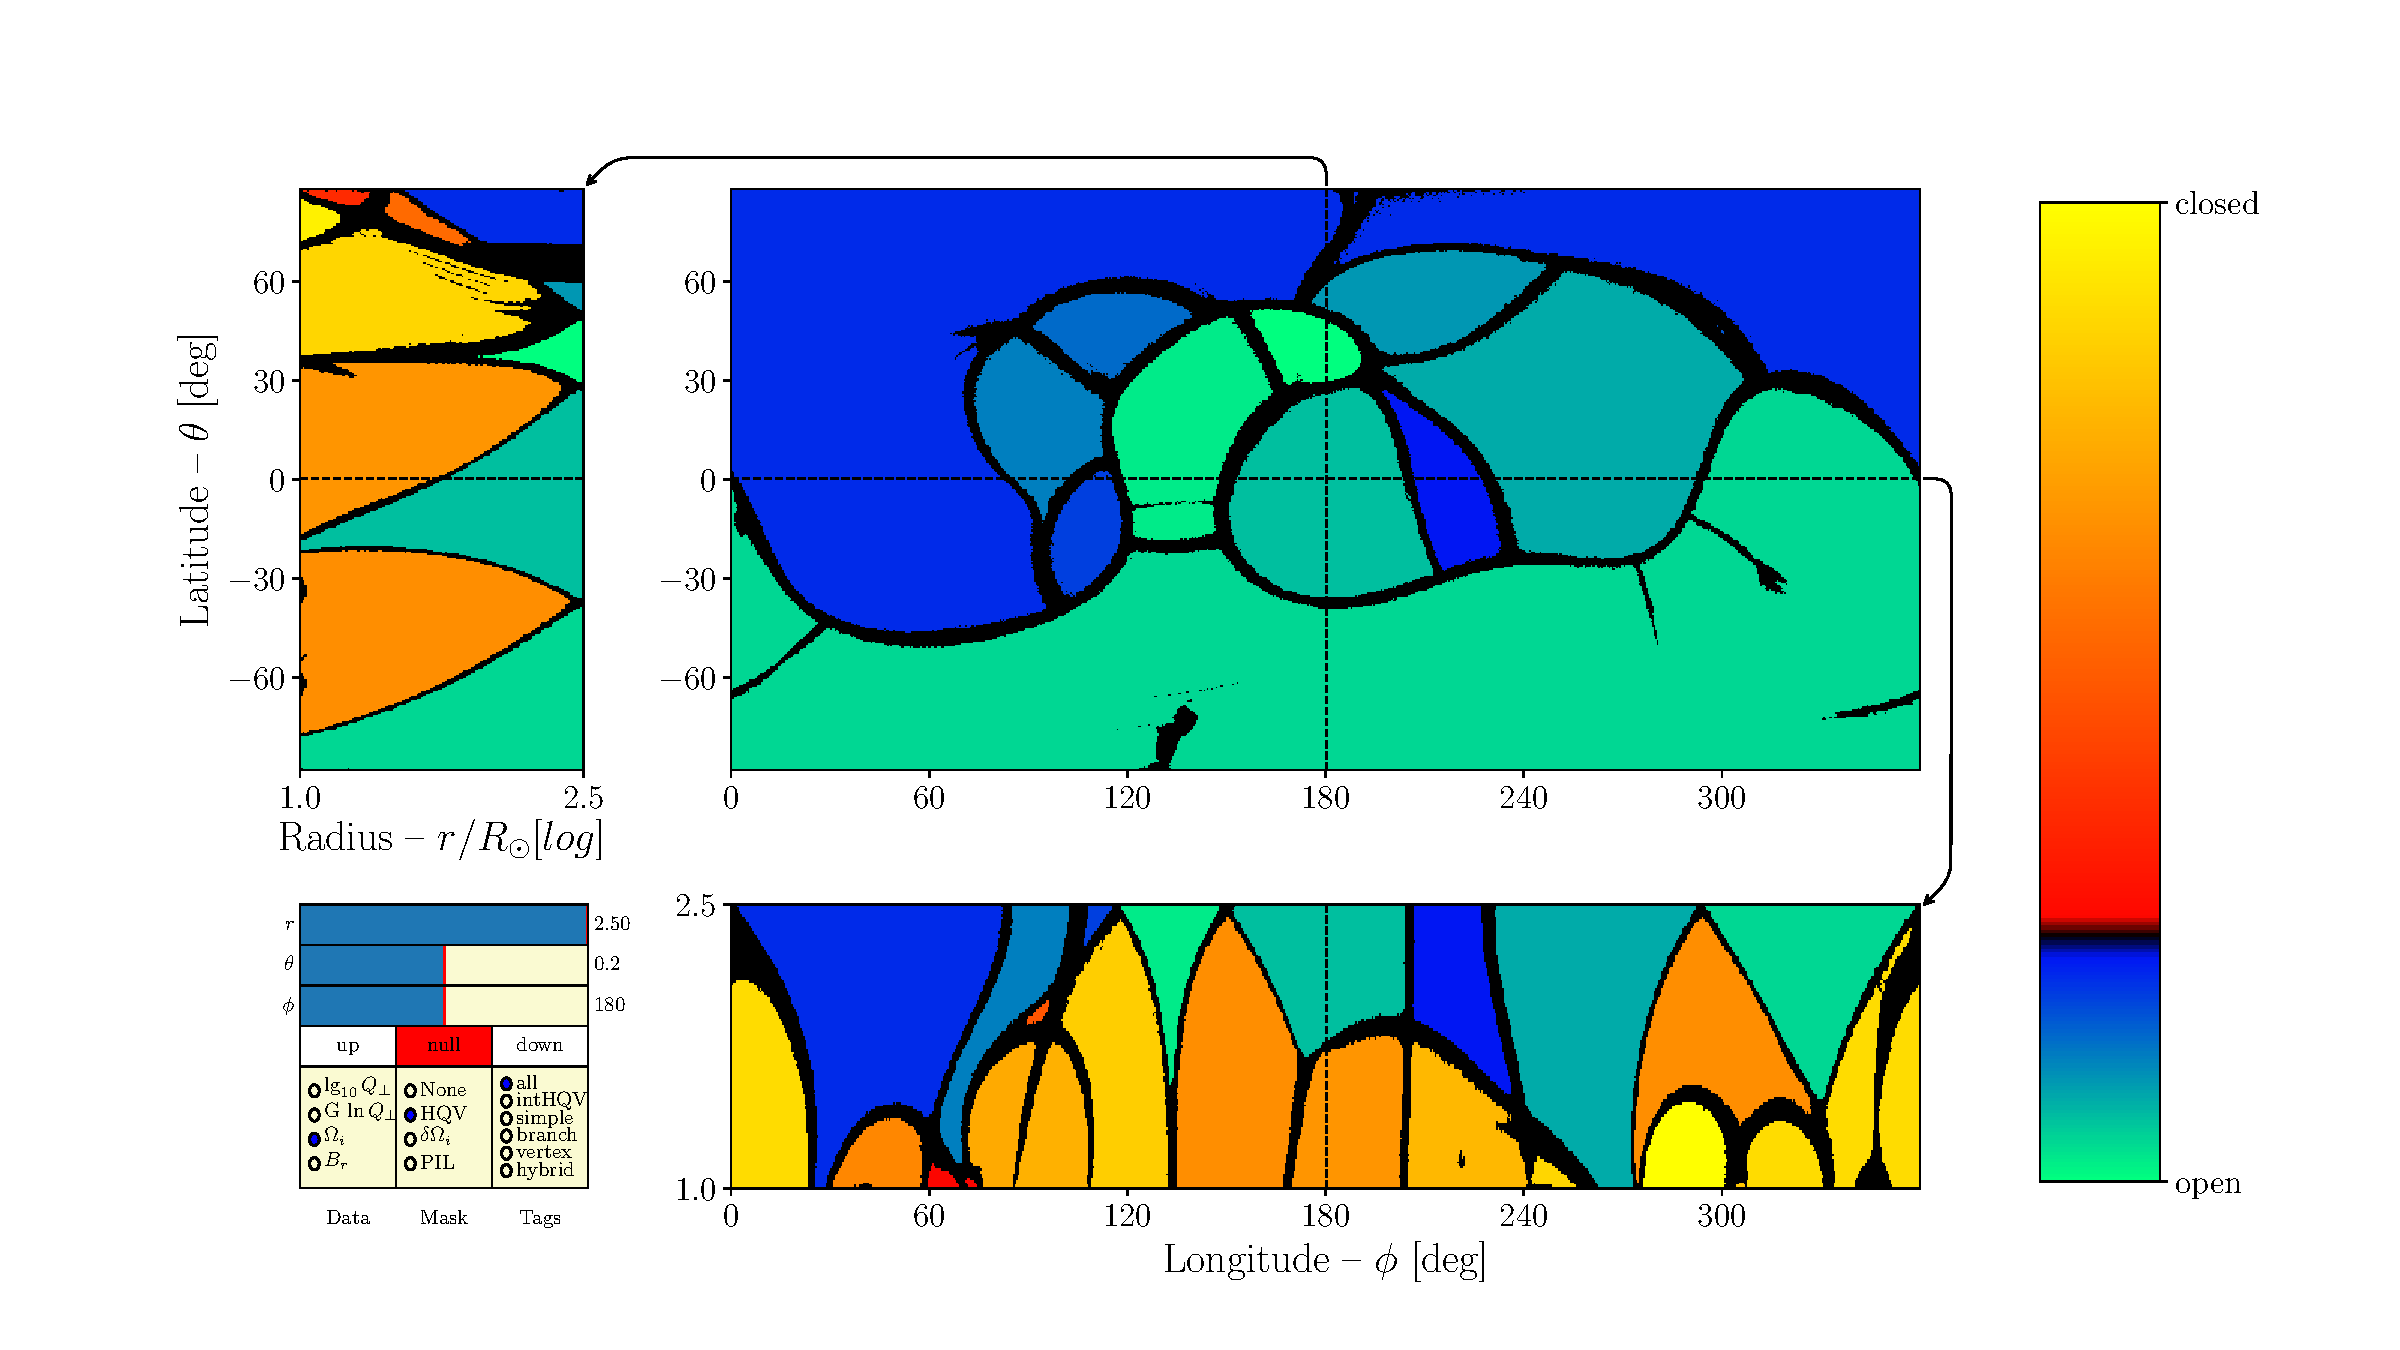
\includegraphics[width=0.49\linewidth]{./fig_src_fls/vis1}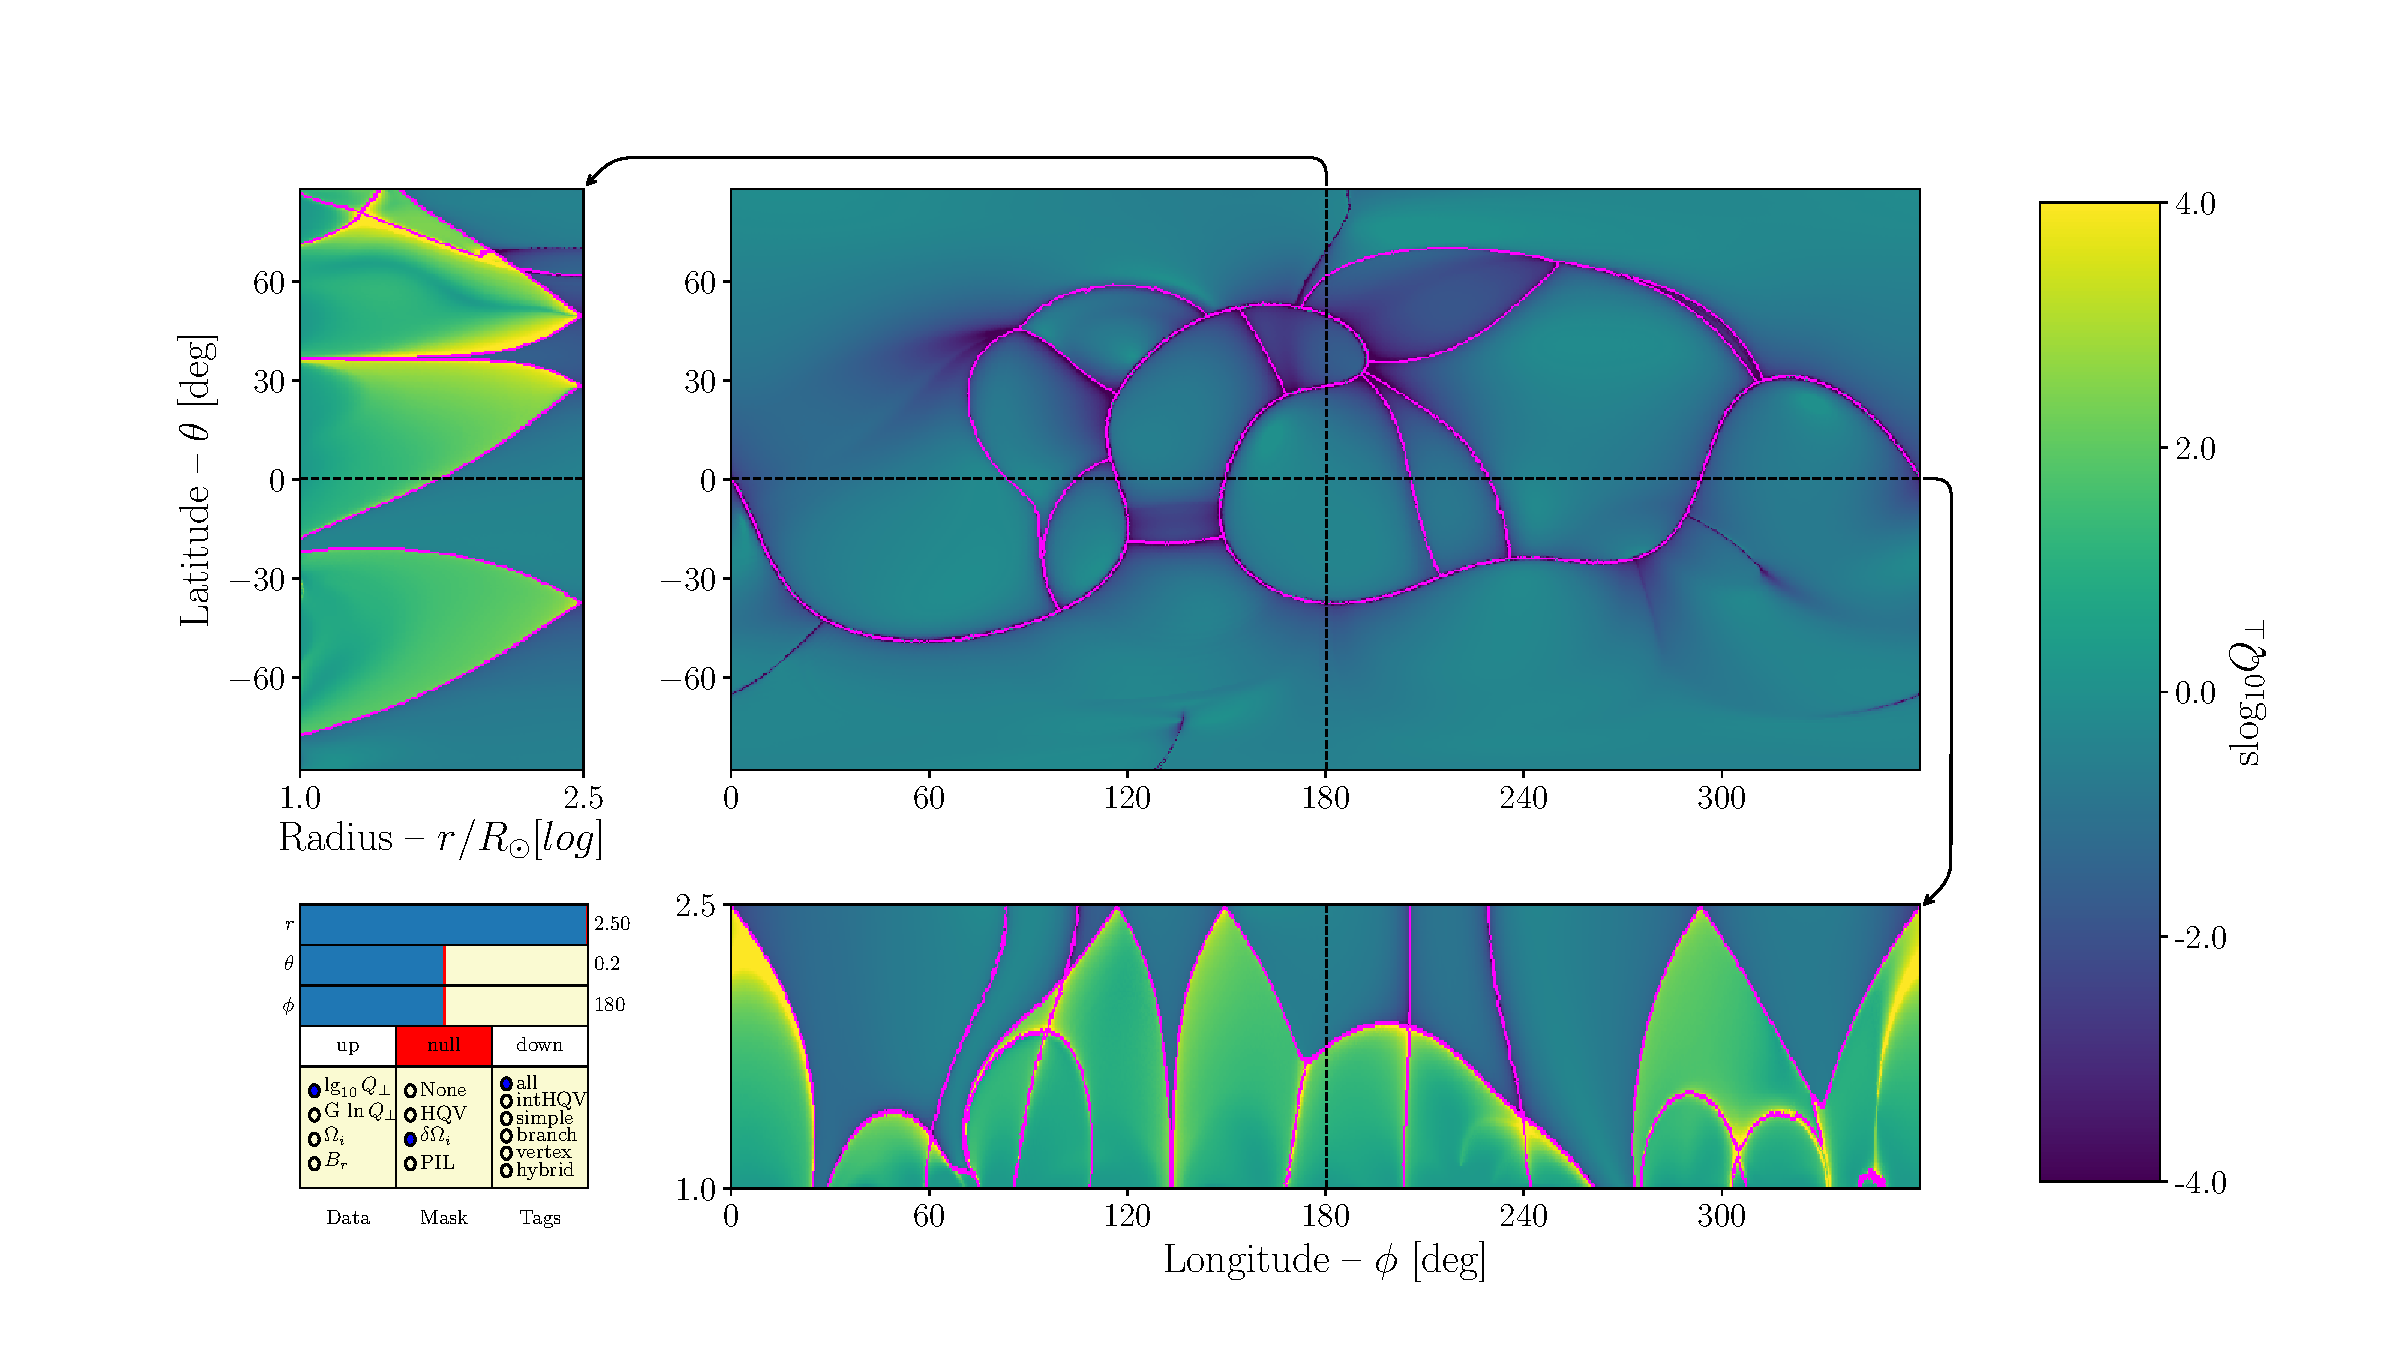
\includegraphics[width=0.49\linewidth]{./fig_src_fls/vis0}\\
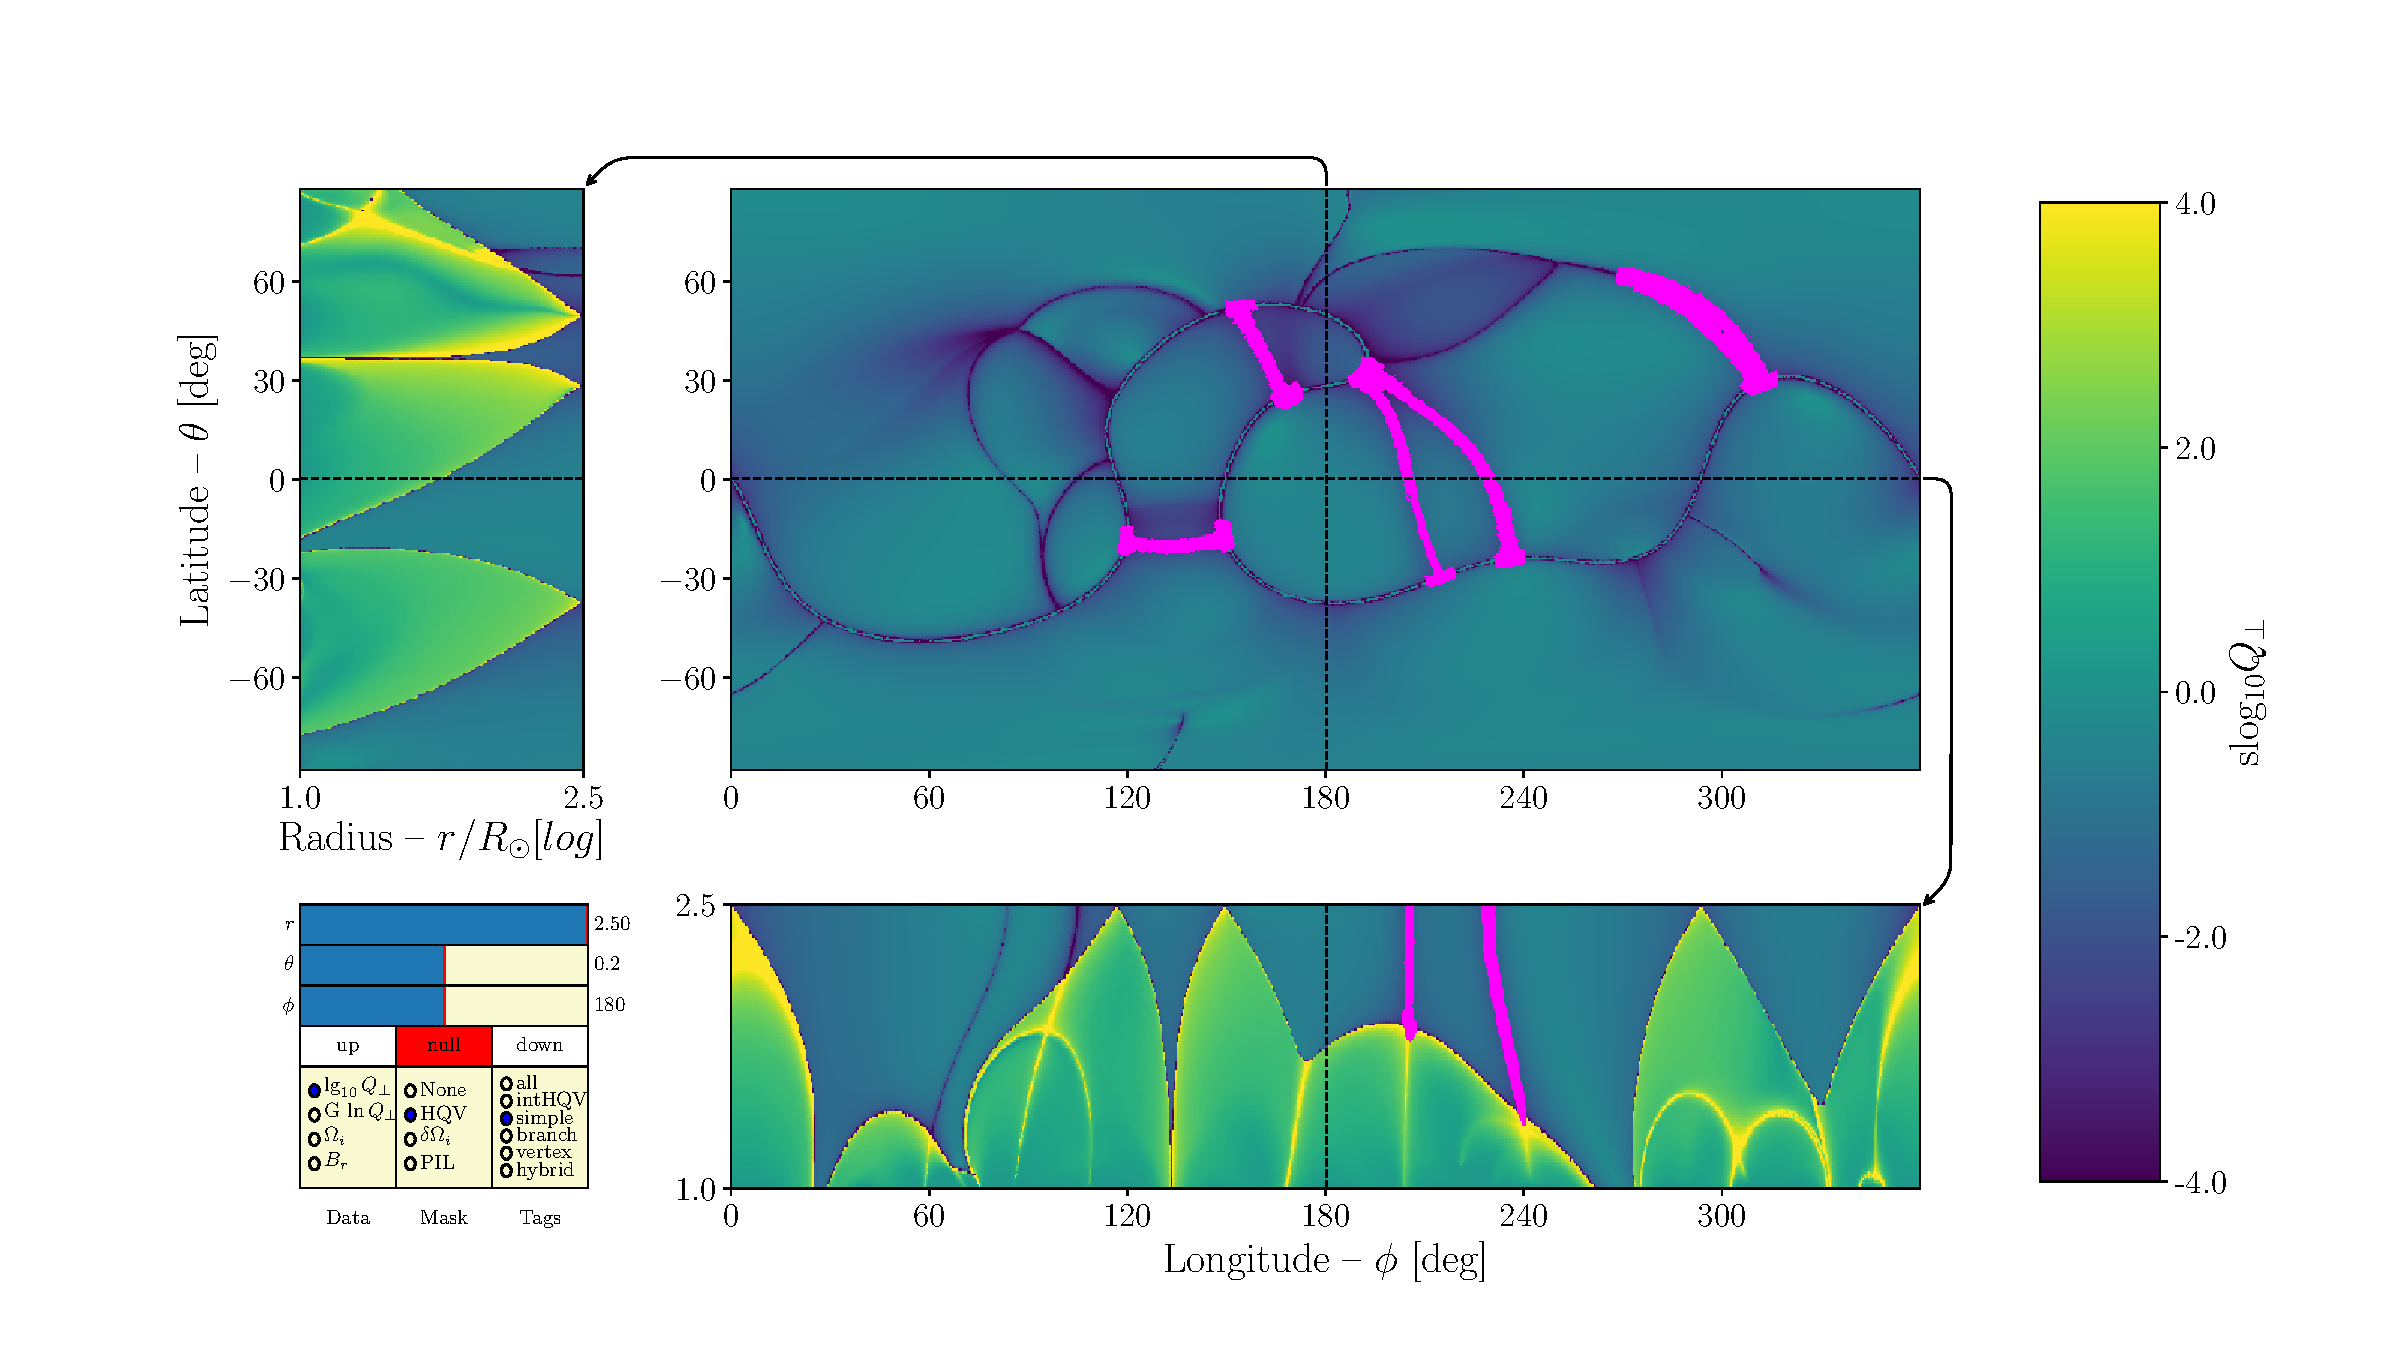
\includegraphics[width=0.49\linewidth]{./fig_src_fls/vis2}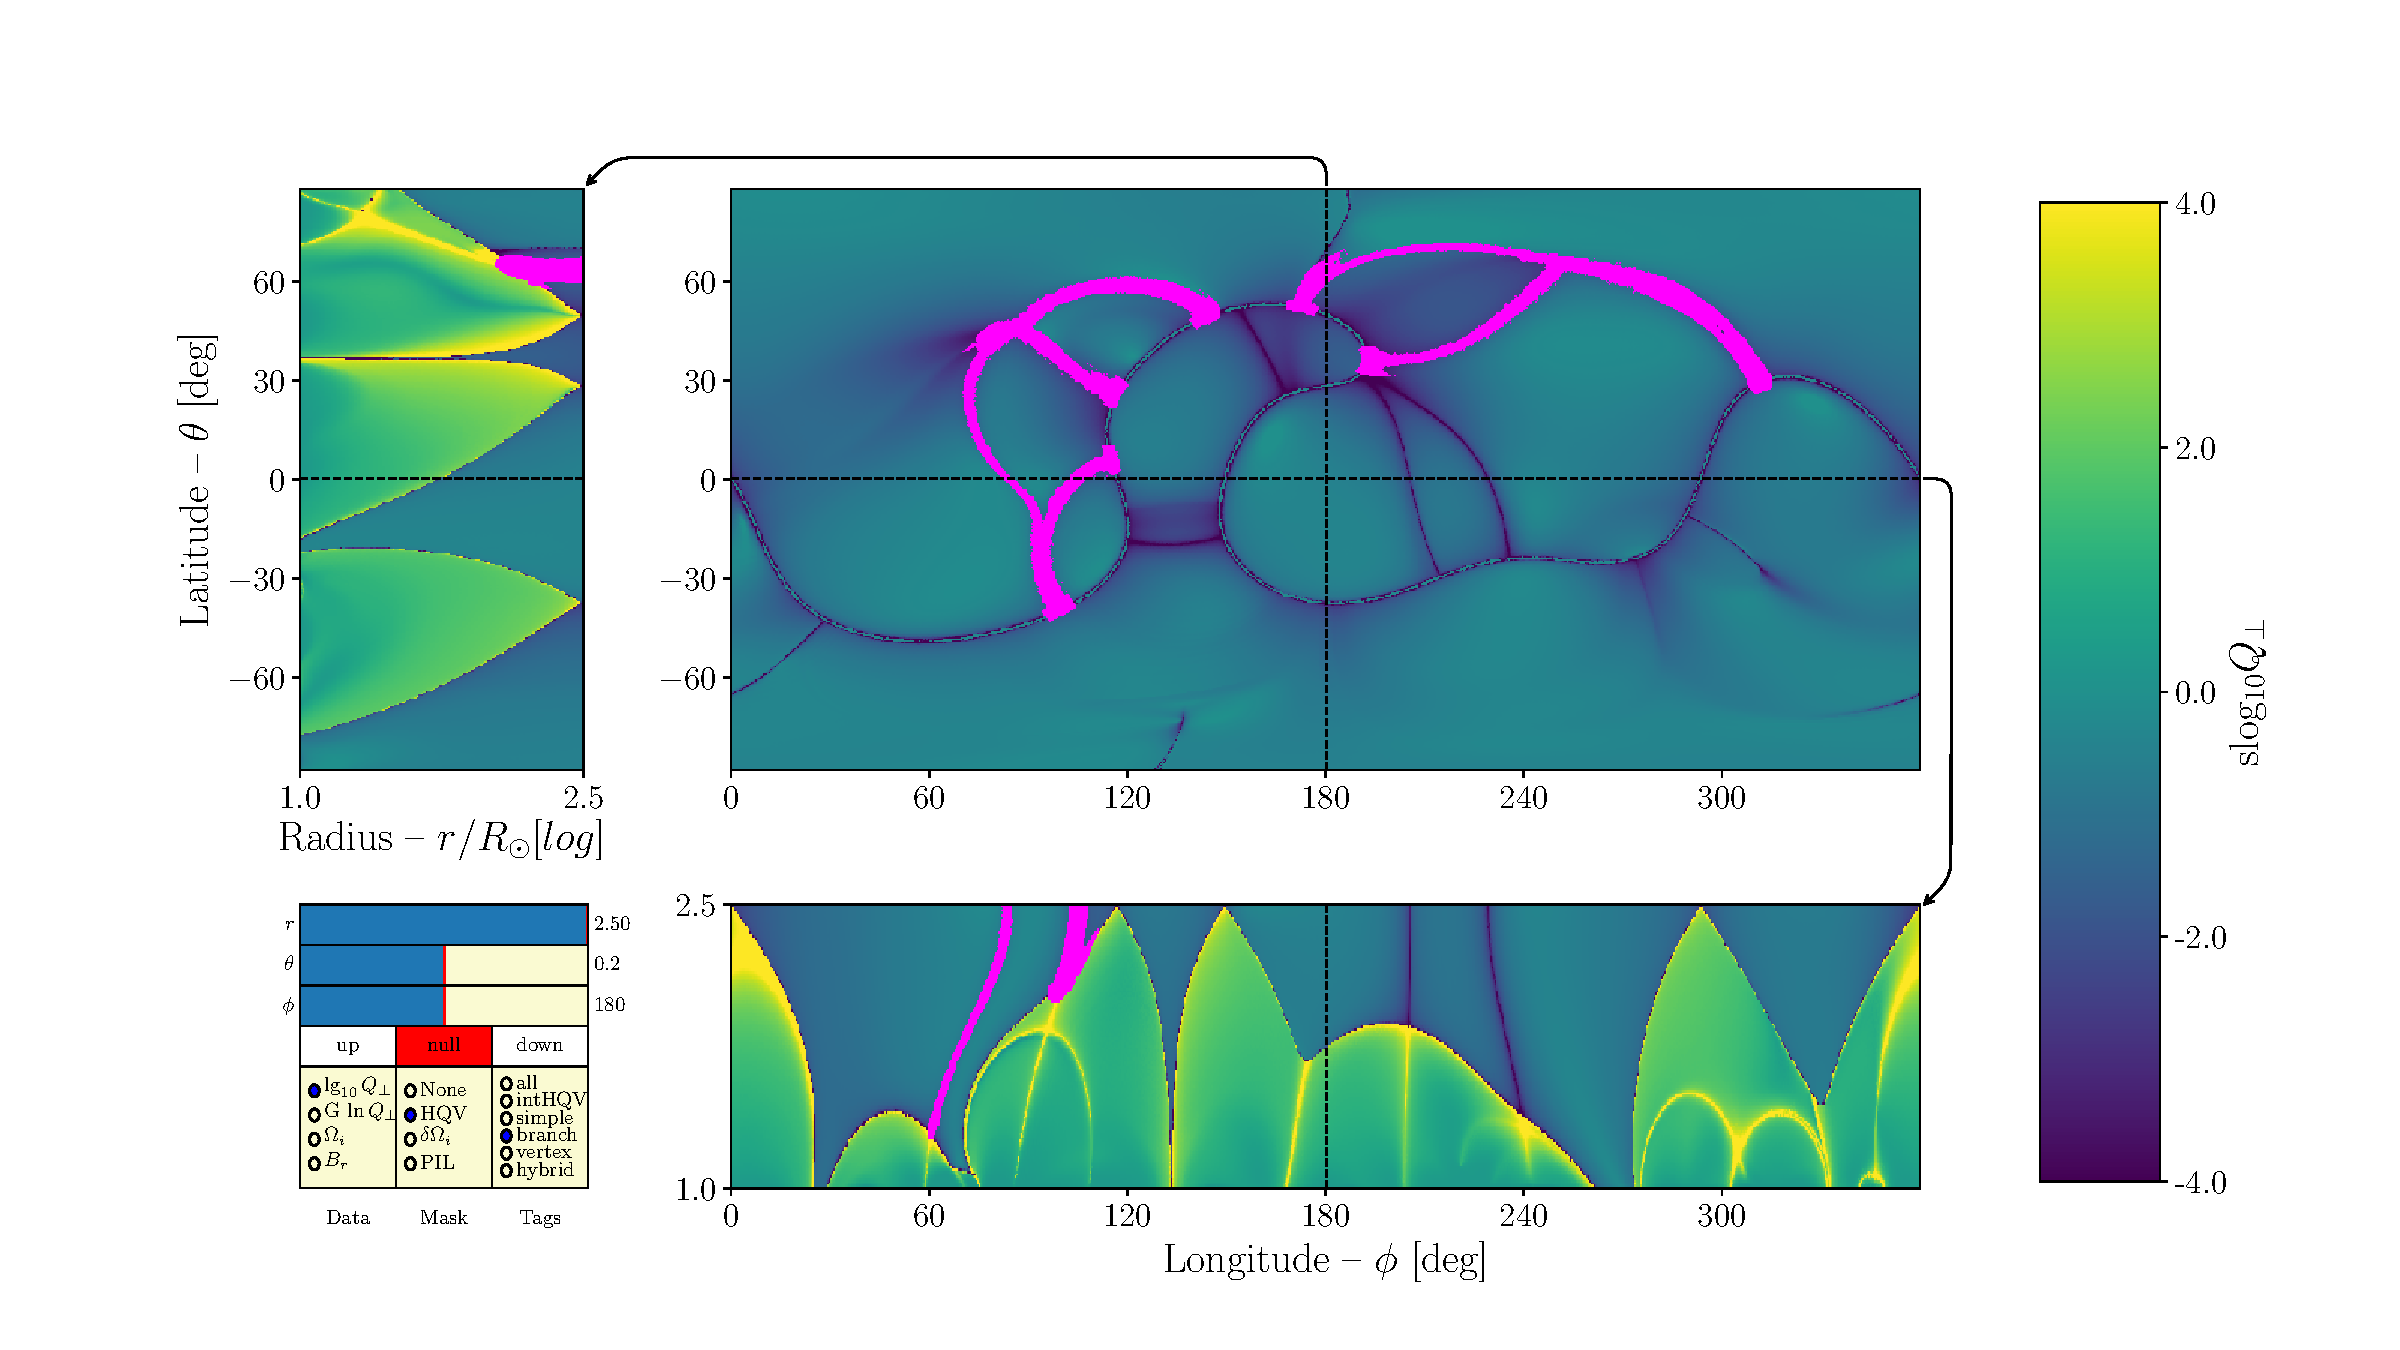
\includegraphics[width=0.49\linewidth]{./fig_src_fls/vis3}\\
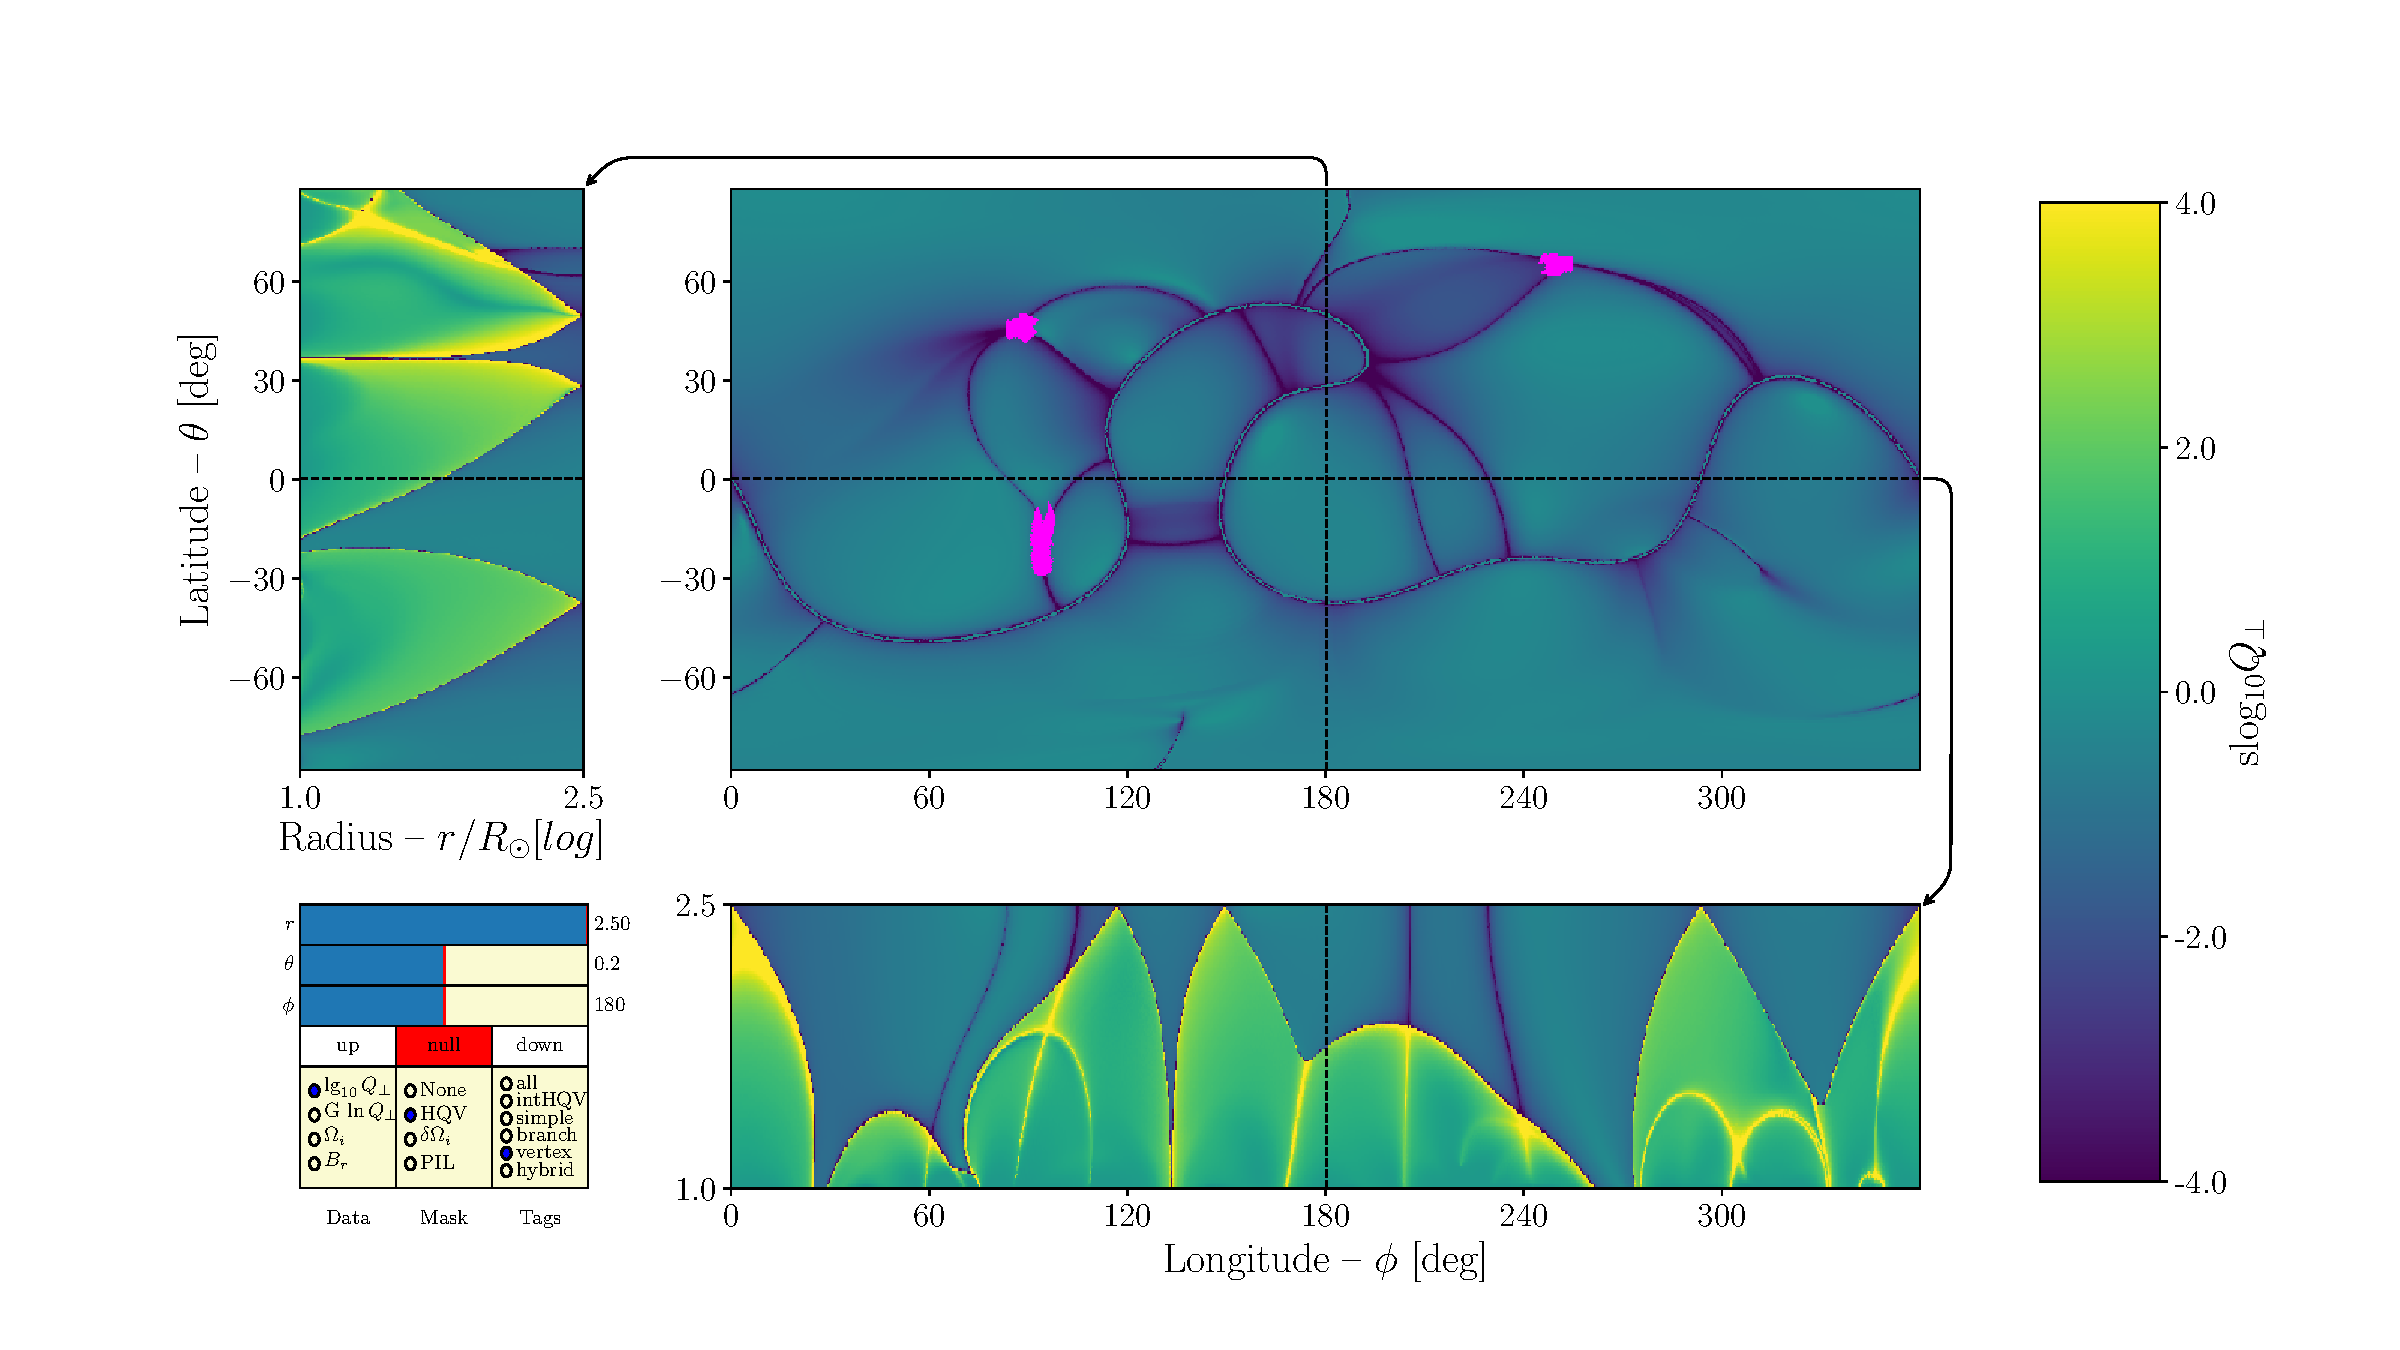
\includegraphics[width=0.49\linewidth]{./fig_src_fls/vis4}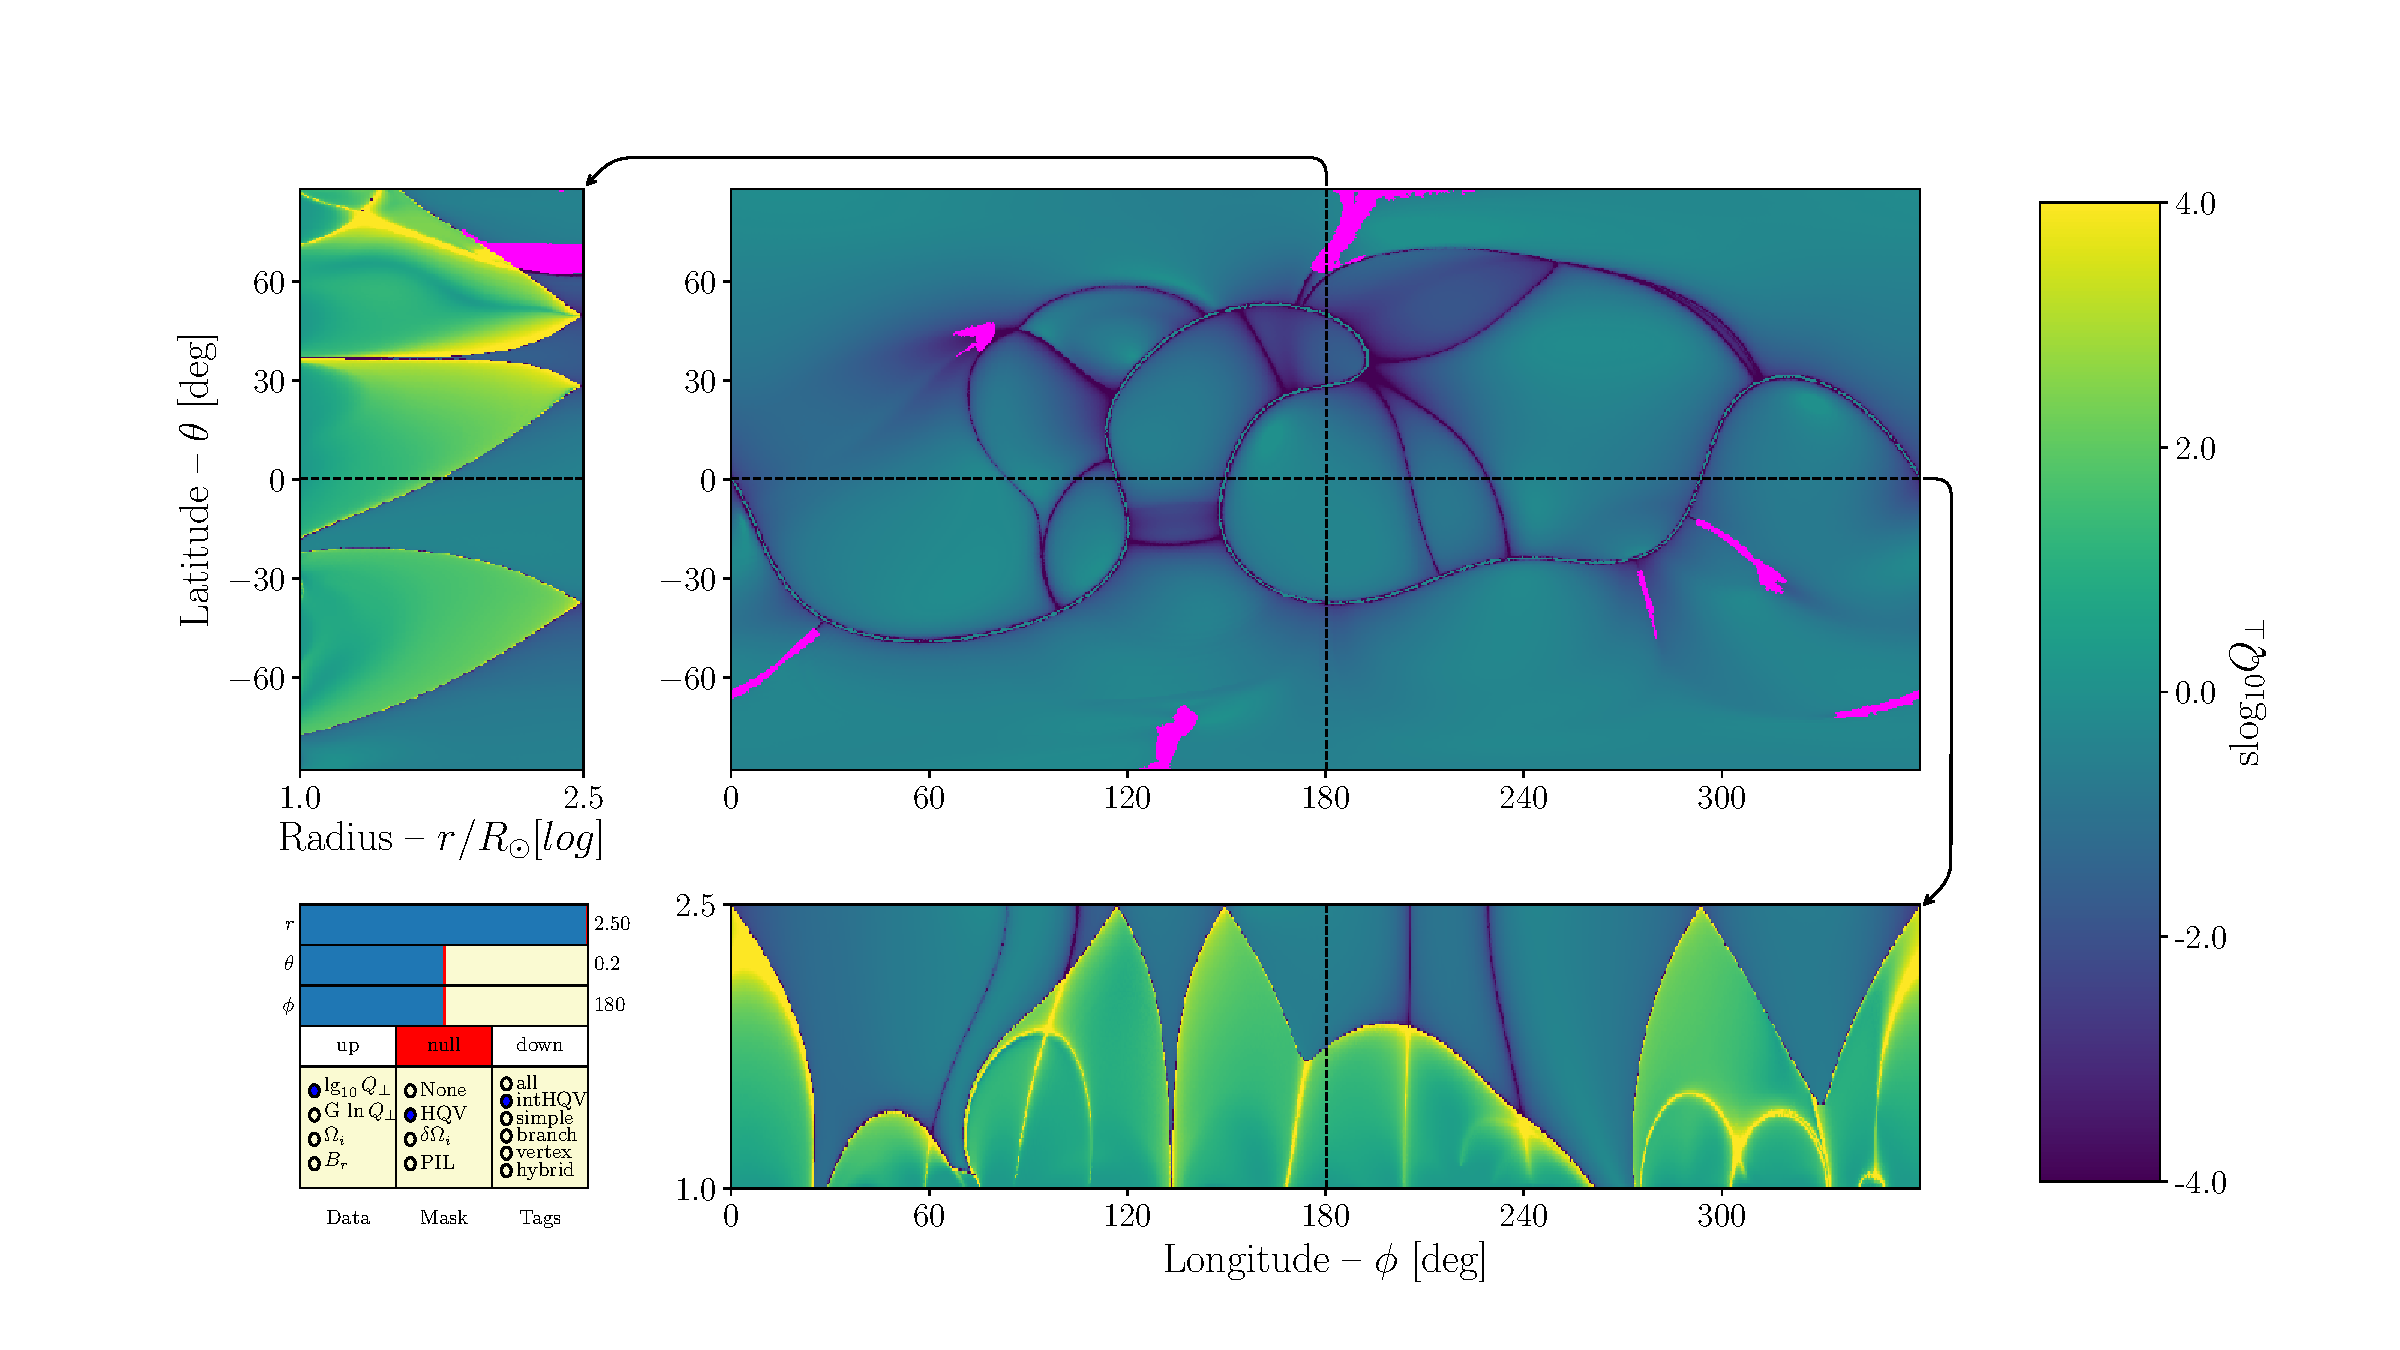
\includegraphics[width=0.49\linewidth]{./fig_src_fls/vis5}
\caption{Visualization of catalogued structures: Segmentation map (tl), $Q_\perp$ map with domain boundaries (tr), $Q_\perp$ map with `simple layers' (cl) $Q_\perp$ map with `branching layers' (cr), $Q_\perp$ map with `vertex lines' (bl), $Q_\perp$ map with interior HQVs ('br').}
\label{vis_opts.fig}
\end{figure}

Following the initial generation of the \path{interior_HQV} and \path{exterior_HQV} attribute lists, we use a combination of routines to determine how each entries associates with other relevant features.
We begin with the \path{Model().get_null_regions_dist()} and \path{Model().get_null_intHQV_dist()} methods, which tabulate distance from every magnetic null to the nearest point in a given domain, or subdomain in the case of interior HQVs. 
After determining the distances to the nulls, the \path{Model().associate_structures()} routine iterates through each entry in \path{interior_HQVs} and \path{exterior_HQVs} and tests to see if either list has entries that are co-spatial with entries from the other list, in which case such associated structures are appended to each others metadata. 
The magnetic nulls are then reordered according to distance from each HQV entry, and vice versa, so that every HQV object contains its own list of magnetic nulls, ordered by distance, and every null contains its own lists of interior and exterior HQVs, again ordered by distance. 
Finally, for each element in \path{exterior_HQVs}, the properties of its various parent and child entries and associated interior HQVs are inspected in detail to determine whether a given HQV structure is to be considered a simple layer, a branching layer, a vertex, or an element of the heliospheric current sheet (HCS) or open-closed boundary (OCB), according to logic developed for consistency with \cite{Scott:2018a}.

As before, we take vertices, simple arc segments, branching arc segments, and detached arc segments, to refer to specific morphological features at the outermost boundary.
Here these structures are generalized to 3-dimensions and we consider their extension into the coronal volume. 
The details of this determination can be rather subtle in some cases, but broadly speaking the logic is as follows:
\begin{itemize}
\item An exterior HQV is considered part of the HCS if the associated label list contains one or more entries from each of \path{result.opos_labels} and \path{result.oneg_labels}.
\item An exterior HQV is considered part of the OCB if the associated label list contains one or more entries from each of \path{result.clsd_labels} and either \path{result.opos_labels} or \path{result.oneg_labels}.
\item An exterior HQV is considered a `vertex line' if is derived from the interface of three or more domains, which merge at a point away from the HCS and OCB, so that it's imprint at the outer boundary is consistent with a `vertex'.
\item An exterior HQV is considered a `branching layer' if it is derived from the interface of a pair of domains and is partially co-spatial with a `vertex line'.
\item An exterior HQV is considered a `simple layer' if it is derived from the interface of a pair of domains and is not at least partially co-spatial with a `vertex line'.
\item Interior HQVs, which do not partition discrete flux domains, form the collection of fully and partially detached high-Q layers, which are distinguished by the properties of their \path{associated_extHQVs}. 
\end{itemize}
The above definitions are a summary of relevant properties of each type; however the exact logic is significantly more complex as it deals with a variety of possible counter-examples, such as, e.g., the intersection of a pair of domains that exists only and entirely within a vertex formed of four or more groups.
 
\section{Miscellaneous}

Execution of the entire model generation begins with first loading the module, and then instantiating a model object as \path{model = HQVseg.Model()}.
The working directory can then be set by \path{Model().inputs.q_dir = 'your_path'}, or by passing the argument \path{'your_path'} as an option to \path{Model().inputs = HQVseg.Inputs(q_dir = 'your_path')}. 
In either case, once the model object has a valid entry for \path{inputs.q_dir}, the various routines can be executed by calling their wrappers: \path{Model().do_import(), Model().do_segment(), Model().do_itemize(), Model().do_inspect()} or with the global wrapper \path{Model().do_all()}. 
Individual models can be written to or read from disc using the \path{Model().save_data()} and \path{Model().load_data()} routines, with either explicit or default filenames.
The save format is handled by \texttt{Numpy's} \path{pickle} method, using a custom file type (\path{Bytefile()}) which executes the write in batches to avoid buffer issues.

Visualization is handled through a GUI that is launched with the command \path{Model().visualize()}.
The GUI shows slices through three different coordinates, set using sliders, and allows stepping through the locations of the magnetic nulls.
Displayed data can be set to $\rm{slog}_{10}Q_\perp$, $\grad \ln Q_\perp$, \path{vol_seg}, or $B_r$, while the mask can be set to `None', \path{hqv_msk}, $\delta \Omega_i$, or `PIL'.
The mask can be further reduced with tags that select the subsets for `all', `interior HQVs', `simple layers', `branching layers', `vertex lines', or `hybrid', which shows layers and interior HQVS that are mutually co-spatial.
Additional visualization can be achieved manually by plotting the various arrays directly, or by calling the \path{Model().export_vtk} method, which accepts various keywords for writing either the entire model or subsets of the model to VTK files, which can be rendered using various routines such as ParaView. 

\begin{figure}
\center
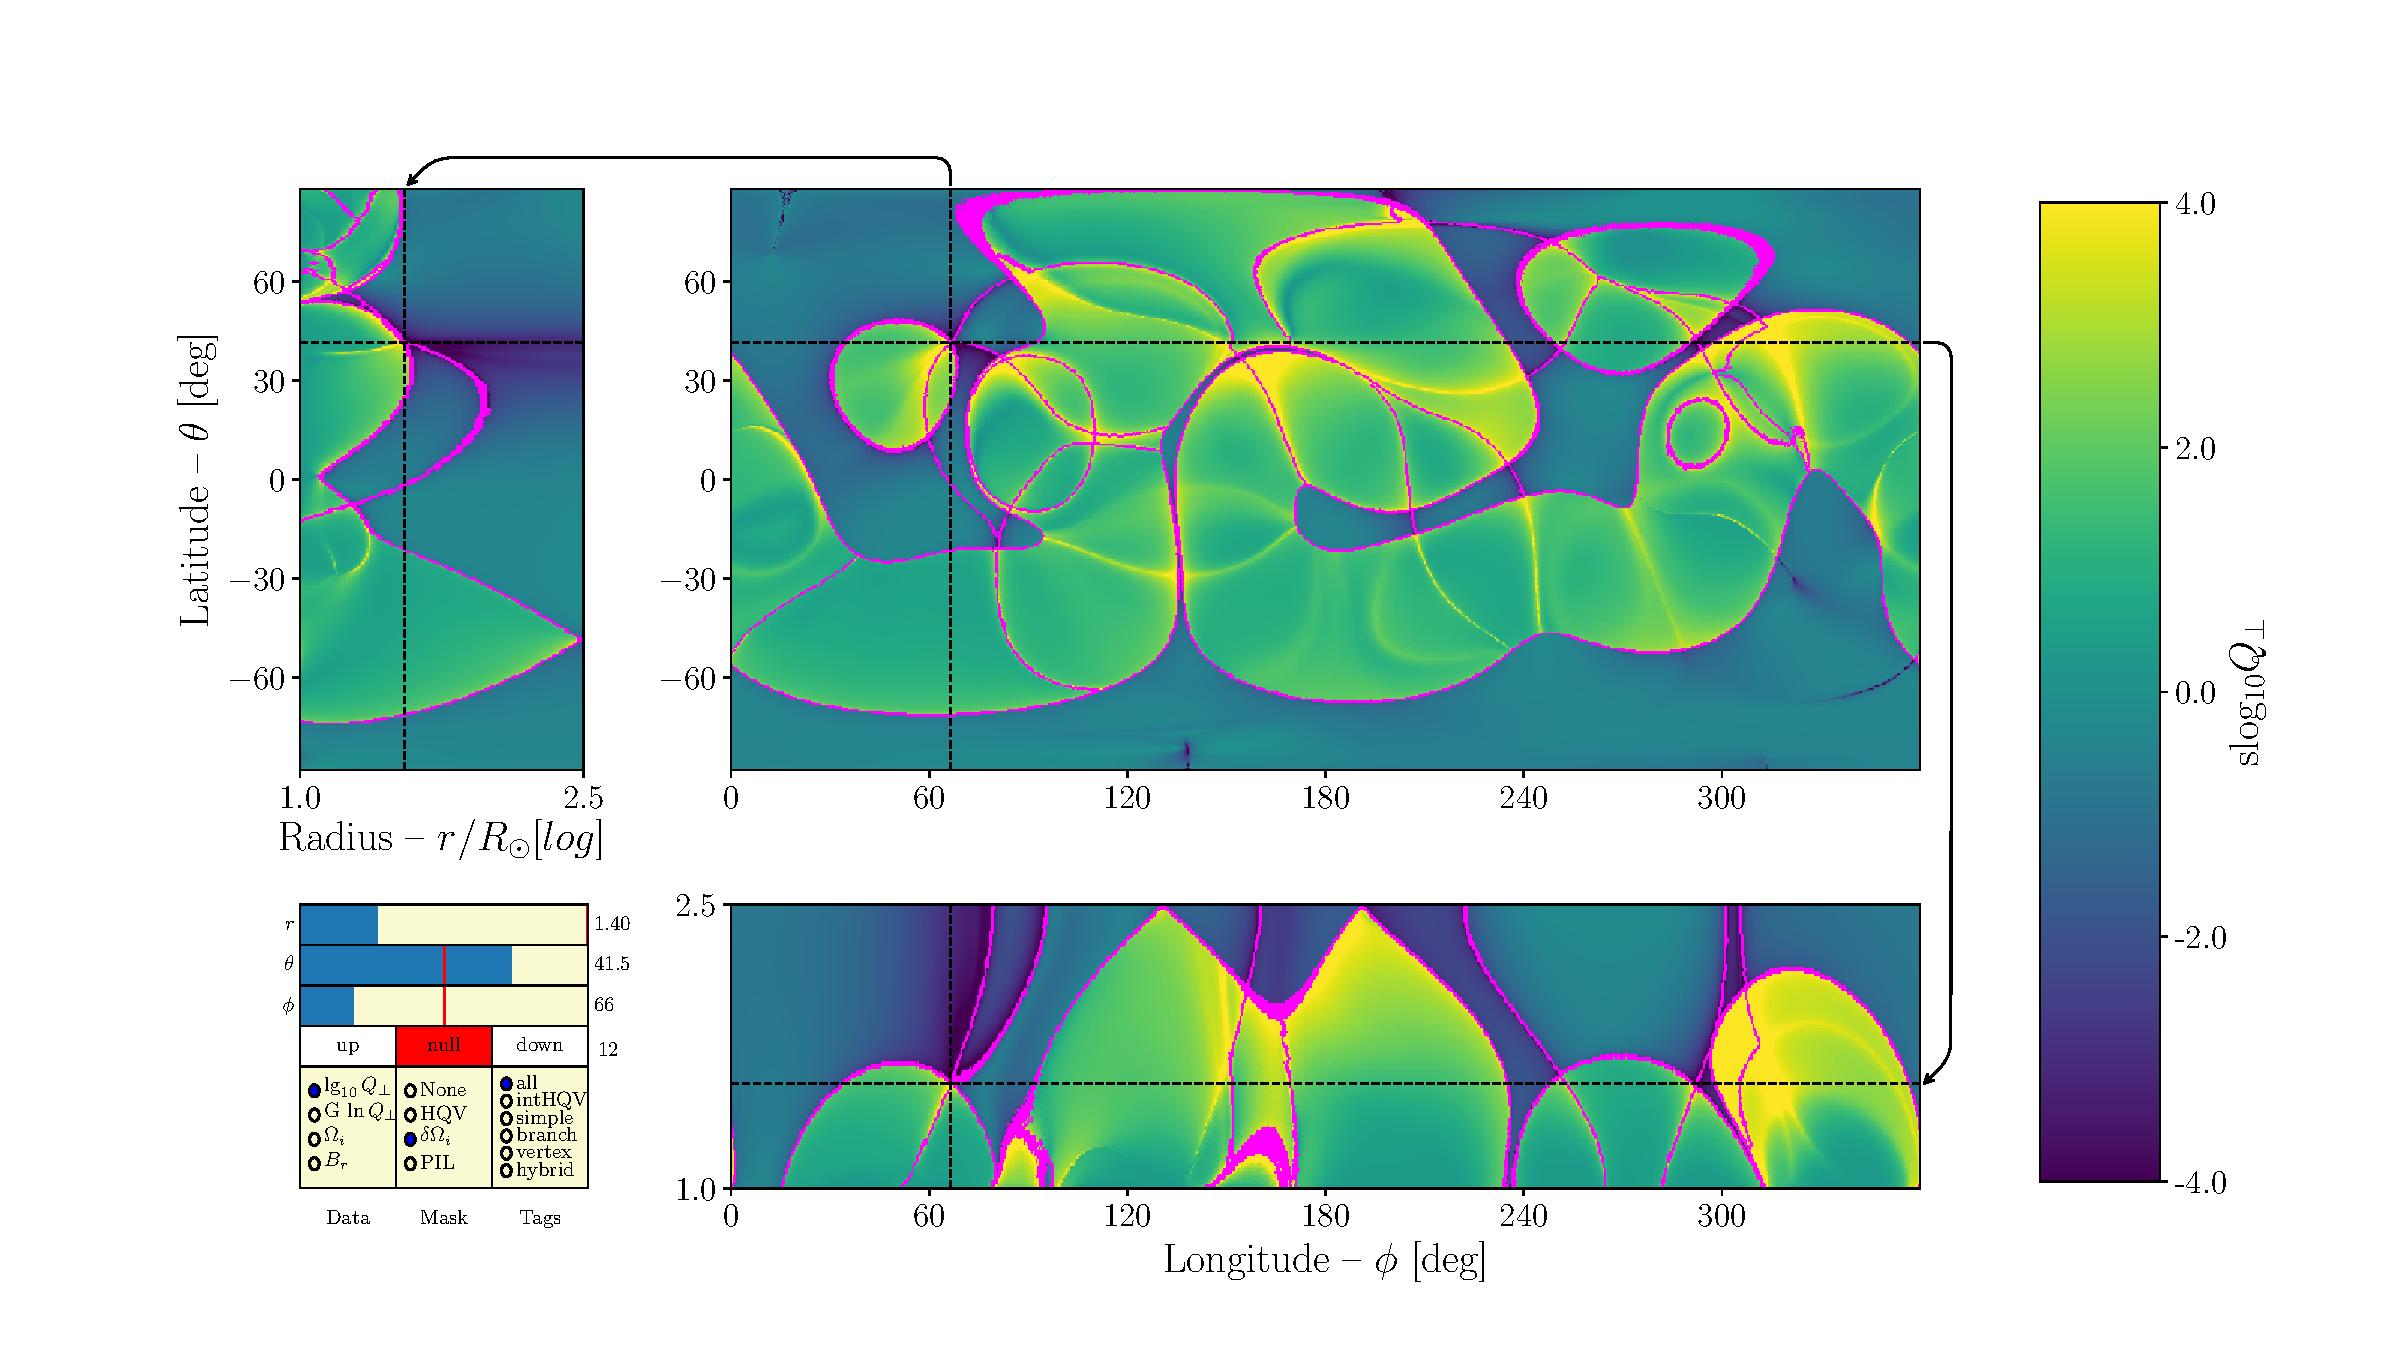
\includegraphics[width=\linewidth]{./fig_src_fls/gui}
\caption{GUI visualization demonstrating slices, masks, and null stepping.}
\label{vis_opts.fig}
\end{figure}



\end{itemize}


\bibliographystyle{apj}
\bibliography{\string~/Dropbox/RBS_big_bib}




%%%%%%%%%%%%%%%%
%%%  Appendix
%%%%%%%%%%%%%%%%


\end{document}



\subsection{PFSS Model Preparation}\label{bfield.sec}

\begin{table}
\begin{tabular}{| l | l | l |}
\hline
Model & Date & GONG datafile\\
\hline
${\bf B}^{(1)}$ & 01 Jan. 2008 & \path{mrbqs080101t0554c2065_258.fits}\\
${\bf B}^{(2)}$ & 01 Jan. 2009 & \path{mrbqs090101t0554c2078_107.fits}\\
${\bf B}^{(3)}$ & 01 Jan. 2010 & \path{mrbqs100101t0554c2092_330.fits}\\
${\bf B}^{(4)}$ & 01 Jan. 2011 & \path{mrbqs110101t0304c2105_194.fits}\\
${\bf B}^{(5)}$ & 01 Jan. 2012 & \path{mrbqs120101t0554c2118_054.fits}\\
${\bf B}^{(6)}$ & 01 Jan. 2013 & \path{mrbqs130101t0424c2132_265.fits}\\
${\bf B}^{(7)}$ & 01 Jan. 2014 & \path{mrbqs140101t0004c2145_129.fits}\\
${\bf B}^{(8)}$ & 29 \,Jul. 2014 & \path{mrbqs140729t2354c2153_237.fits}\\
${\bf B}^{(9)}$ & 01 Jan. 2015 & \path{mrbqs150101t0004c2159_352.fits}\\
${\bf B}^{(10)}$ & 01 Jan. 2016 & \path{mrbqs160101t0014c2172_214.fits}\\
${\bf B}^{(11)}$ & 01 Jan. 2017 & \path{mrbqs170101t0004c2185_064.fits}\\
\hline
\end{tabular}
\caption{GONG Magnetogram dates for PFSS models.}\label{date-obs.tab}
\end{table}

The model magnetic field is developed in the same manner as described in \cite{Scott:2018a}, beginning with GONG magnetogram data taken from eleven different samples between 2008 and 2017. 
To distinguish these models, we shall refer to each with a superscript index following the convention that ${\bf B}^{(i)}$ is the $i$-th model magnetic field, with the corresponding observation dates given in Table \ref{date-obs.tab}. 
The same convention will be used to distinguish quantities that are derived from ${\bf B}^{(i)}$, with the understanding that if the superscript is omitted, the discussion applies in general. 
As in the previous study, each field is constructed from a potential field source surface (PFSS) model, with the source magnetogram data smoothed by a pseudo-gaussian filter with a characteristic fall-off at angular wave number of $l_f \sim 18$. 
The model dimensions are $61 \times 180 \times 360$ in log-radius, sine-latitude, and longitude, respectively. 

\begin{figure}[h]
\center
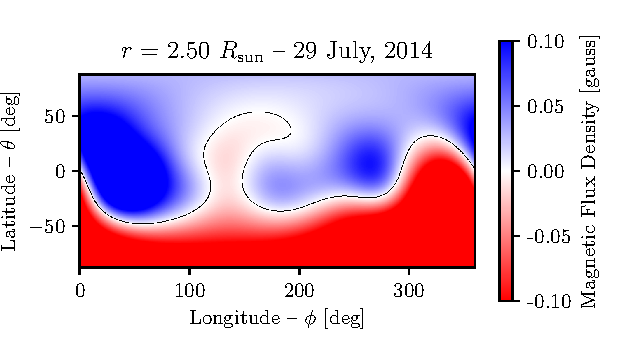
\includegraphics[width=\linewidth]{./fig_src_fls/140729_br_top.pdf}
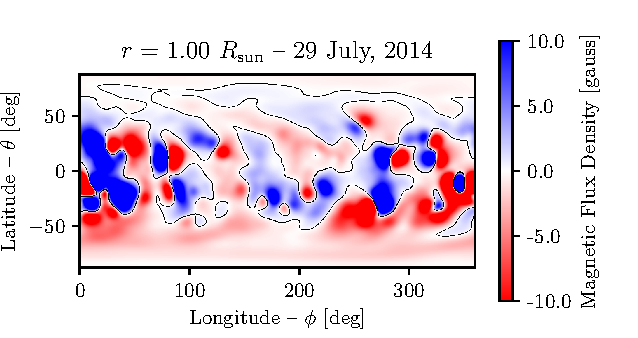
\includegraphics[width=\linewidth]{./fig_src_fls/140729_br_bot.pdf}
\caption{Radial magnetic field ${\bf B}^{(8)}$ from 29 July 2014. The top and bottom panels represent the source surface ($r=2.5 R_{\rm sun}$) and photospheric ($r=1.0 R_{\rm sun}$) boundaries. Data is smoothed with a  pseudo-gaussian filter of the form $f = exp(-l(l+1) k)$, with $k=0.002$. The field is then interpolated onto a grid with the same dimensions as $Q$ (see section \ref{squash.sub}) for consistency. }
\label{source_field.fig}
\end{figure}

The radial component of ${\bf B}^{(8)}$ is shown at the inner and outer radial boundaries in Figure \ref{source_field.fig}.
The positive and negative polarity domains are indicated in blue and red, with weak field regions appearing as white.
The black curves indicate the location of polarity inversion lines, of which there is only one at the source surface ($r=2.5 R_{\rm sun}$), this being the base of the heliospheric current sheet.

I would like to make reference to Figure \ref{source_field.fig}.

\subsection{Squashing Degree}\label{squash.sub}

\begin{figure*}
\center
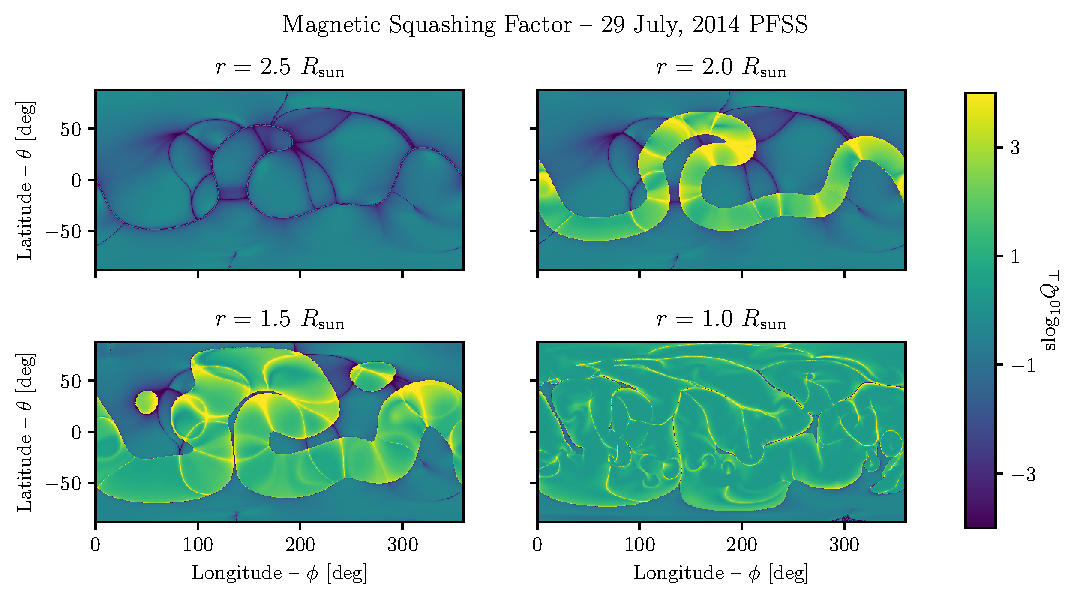
\includegraphics[width=\linewidth]{./fig_src_fls/140729_slog10q_multi.pdf}
\caption{Sign $\log_{10} Q$ at radial heights of $r = \{1.0, 1.5, 2.0, 2.5\} R_{\rm sun}$ for 29 July, 2014 PFSS. Dark colors indicate open flux, corresponding to coronal holes at the lower boundary. Dark bands at the upper boundary indicate the intersections of QSLs with the source surface. The yellow curve in the top panel shows the apex of the helmet streamer, just below the heliospheric current sheet.}
\label{slog10q_multi.fig}
\end{figure*}

For each model field ${\bf B}^{(i)}$ the corresponding magnetic squashing factor $Q^{(i)}$ is calculated using the \path{qslSquasher} routine \citep{Tassev:2016, Scott:2017a}.
For this project the code has been configured to run on an Linux based desktop computer hosting an nVidia Tesla k40 GPU.
We use trilinear field line tracing with an Eulerian integration step size of 0.25 Mm (equivalent to 20 steps per grid cell of the source field). 

The output grid is uniformly spaced in angular coordinates and exponentially spaced in the radial coordinate. 
The grid resolution is 120 x 480 x 960 in radius ($r$), north latitude ($\theta$), and longitude ($\phi$), respectively.
The domain is periodic in $\phi$, with $1\le r \le 2.5$ and $|\theta| \le 88^\circ$. 

Since the squashing factor is a positive definite quantity, whose minimum theoretical value is $Q_{\rm min} = 2$, we can adopt the functional representation 
\begin{equation}
{\rm slog}_{10} Q^{(i)} = \pm \log_{10} Q^{(i)},
\end{equation}
such that ${\rm slog}_{10} Q^{(i)}$ is positive or negative where the field lines of the associated mapping are closed or open. 
An advantage of this representation is that the separatrix surface of the open-closed boundary (OCB) is bounded on either side by regions of opposite signed ${\rm slog}_{10}Q$, so not only is $Q$ large (formally infinite) along the OCB, but so too is the gradient of ${\rm slog}_{10}Q$.
Note that this differs from the convention of some other authors, who use the sign of $Q$ to denote the polarity of the magnetic field at the boundary of the domain.

A depiction of ${\rm slog}_{10}Q^{(8)}$ is given in Figure \ref{slog10q_multi.fig}, which shows constant-radius slices through the volume at radial heights of $r=\{2.5, 1.6, 1.0\} R_{\rm sun}$. 
Dark blue and light yellow regions indicate highly squashed flux in the open and closed domains, respectively. 
The open-closed boundary (OCB) is located at the sharp transition between the extremes of the color-scale.
The OCB is the only structure than can be definitively identified as a topological feature since it necessarily partitions distinct flux domains 
-- all other structures may be either separatrix surfaces or quasi-separatrix layers, depending on the presence of magnetic nulls, which must be found explicitly. 

\subsection{Coronal Volume Segmentation}\label{vol_seg.sec}

The operating assumption for the volume segmentation approach is that large values of $Q$ (or $|\nabla Q|$) delineate high-Q volumes (HQVs), which may in turn be either separatrix surfaces or quasi-separatrix layers (QSLs). 
In either case these serve as boundaries for low-Q volumes that correspond to magnetic flux domains. 
We therefore proceed by attempting to divide the numerical domain into sub-volumes whose boundaries lie within the identified QSLs. 
The process therefore depends on our ability to accurately identify quasi-separatrix layers.  

\begin{figure}
\center
\includegraphics[width=\linewidth]{fig_src_fls/140729_sobel_top.pdf}
\includegraphics[width=\linewidth]{fig_src_fls/140729_mask_top.pdf}
\caption{Sobolev Norm and thresholded mask for ${\rm slog}_{10}Q_\perp$ at $r=2.5R_{\rm sun}$ from 29 July, 2014 PFSS. The mask threshold is set to $|{\bf S}(Q_\perp)| > 10^\wedge3.4$.}
\label{sbn_msk.fig}
\end{figure}

\begin{figure*}[ht]
\center
\includegraphics[width = \textwidth]{./fig_src_fls/140729_seg_multi.pdf}
\caption{Discrete domain segmentation for 29 July 2014 at four elevations, from inner to outer boundary. Warm colors (positive labels) represent closed flux domains while cool colors (negative labels) represent open flux domains. Domain boundaries (accentuated in black) are nominally coincident with 3-dimensional ``ridges'', within the interior of the QSLs.}
\label{seg_levels.fig}
\end{figure*}

We begin by defining a mask according to the boolean threshold $|{\bf S}| > S_t (= 10^\wedge4)$, where ${\bf S}$ is a dimensionless Sobolev vector;
\begin{equation}
{\bf S}(Q) = \left( Q, r^2 (\grad \ln Q)^2 \right),
\end{equation}
with $r$ being the radial coordinate and $\grad$ the finite difference approximation to the spatial gradient (with second order center difference in the interior of the domain and first order off-center different at the boundaries). 
Since $Q$ is, itself, dimensionless, ${\bf S}$ can be thought of as a measure of the local spacial complexity of $Q$, which contains information about both its magnitude and its spacial variation -- 
the latter is key when working with the perpendicular squashing factor, for which bald-patch separatrices appear not as singularities in $Q$, but rather as finite discontinuities that are easily located through edge detection. 
Having constructed the mask, $M_S$, based on thresholding of ${\bf S}$, we then apply a morphological closing to remove small holes that are taken to be numerical artefacts. 



With the mask in place, we then apply the \path{\path{distance_transform_edt}} operation from the \path{SciPy} \citep{SciPy} \path{ndimage} module to calculate the distance from every unmasked pixel to the nearest QSL ($d_{\rm qsl}$), and likewise the distance from every masked pixel to the nearest low-$Q$ flux domain ($d_{\rm flx}$). 
From these we define a padded low-Q flux volume as the volume satisfying
\begin{equation}
V_{\rm flx} = \{ r \in \Omega ~ | ~ d_{\rm qsl} > 2 \bar{d_{\rm flx}} \},
\end{equation}
that is, the collection of all points where the distance from the nearest QSL is greater than the characteristic width of a QSL. 
This volume is then discretely labeled using the \path{skimage.label} routine \citep{SciPy}, which divides the domain into simply connected subdomains. 
The domain labeling is performed separately on open and closed flux, with positive integer labels given to closed flux domains, taking the same convention employed for ${\rm slog}_{10} Q$. 
The volume of each domain is compared to a threshold and the domain label is removed if the volume is too small ($< (2~\bar{d_{\rm flx}})^3$) or if the flux domain does not have a footprint on one of the boundaries. 

With the padded volume labeled, it remains to partition the remaining unlabelled volume, including the high-Q regions that must themselves form a part of the segmented coronal volume. 
This is done in a few steps, using the \path{skimage.morphology.watershed} routine \citep{SciPy}, which takes the pre-existing domain labels as seeds and then grows each volume into the unlabelled region while attempting to place region interfaces at ridges or boundaries in the scalar measure ($|{\bf S}(Q_\perp)|$ in this case). 
The desired affect is achieved by growing open and closed flux domains separately, first leaving the QSL mask in place (so as to grow into the padded volume only), and then removing the QSL mask to let each domain expand into its enclosing high-Q boundary. 
Finally, as a last step, the watershed is repeated with no masks, treating open and closed flux simultaneously, which allows for the assignment of region labels to undetermined flux domains (e.g. where the value of $Q$ is junk and the flux cannot be clearly identified as open or closed). 

Once the entire volume has been labeled, it remains to identify domains across the periodic ($\phi=0$) boundary. We do this by comparing the $\phi=0$ and $\phi=2\pi$ slices, and checking for mutually correlated domains on either side. 
For each domain, a mask is created on both sides of the boundary. The masks are multiplied together pairwise. 
If the area of the multiplied masks is greater than 0.75 of the area of the smaller of the two individual masks, then the regions are considered to be paired, and are assigned the same common label. 
This process is performed separately on open and closed flux regions, although the possibility of mislabeling in this manner is extremely low. 

\subsection{GUI}
\begin{figure*}
\center
\includegraphics[width=\linewidth]{./fig_src_fls/gui-crop.pdf}
\caption{Sign $\log_{10} Q$ at radial heights of $r = \{1.0, 1.5, 2.0, 2.5\} R_{\rm sun}$ for 29 July, 2014 PFSS. Dark colors indicate open flux, corresponding to coronal holes at the lower boundary. Dark bands at the upper boundary indicate the intersections of QSLs with the source surface. The yellow curve in the top panel shows the apex of the helmet streamer, just below the heliospheric current sheet.}
\label{slog10q_gui.fig}
\end{figure*}

\subsection{Interface Identification}

\subsection{Specific Configurations}

\section{Results}

Results:
\begin{itemize}[label=$\square$]
	\item{tabulation of arc types}
	\item{tabulation of vertex lines}
	\item{comparison to null detection}
	\item{field line tracing?}
\end{itemize}

\section{Discussion}

Discussion:
\begin{itemize}[label=$\square$]
	\item{Relative importance of various structures?}
	\item{List of configurations to model?}
\end{itemize}
	
\section{Acknowledgements}\label{acknowledgements.sec}

In which I acknowledge support and assistance.

%%%%%%%%%%%%%%%%
%%%  Bibliography
%%%%%%%%%%%%%%%%

